%\documentclass[12pt]{article}
%\usepackage{amsmath}
%\usepackage{mathptmx}
%\usepackage{setspace}
%\usepackage{amssymb}
%\usepackage{float}
%\usepackage{graphicx}
%\usepackage{booktabs}
%\usepackage{subfigure}
%\usepackage[margin=2.5cm]{geometry}
%\usepackage[title]{appendix}
%\usepackage{bm}
%\usepackage{tcolorbox}
%\usepackage{apacite}
\onehalfspacing
%\usepackage{longtable}
%\usepackage{diagbox}
%\usepackage{pdflscape}
%\usepackage{rotating}
	%\usepackage{subcaption}
%	\usepackage{floatrow}



%\usepackage{fontspec}
%\setmainfont{Times New Roman}
\addtolength{\jot}{0.1em}
\linespread{1}
\graphicspath{{./plot/}}


%\begin{document}
%	\section{Strength Comparison Tables}\label{strength_table}

\begin{landscape}
			\section{Empirical Application Result}
			\subsection{Factor Strength Estimation Table}\label{strength_table}
\begin{footnotesize}
\setlength{\tabcolsep}{2pt}
\singlespacing
\centering



		\begin{longtable}{l|lcc|lcc|lcc}

			
					\caption{Comparison table of estimated factor strength on three different data sets, from strong to weak}\label{table:three_ranked_compare}\\

			\hline
			\hline
\multicolumn{1}{l|}{} & \multicolumn{3}{c|}{Ten Year Data}                                                                                                                                                                         & \multicolumn{3}{c|}{Twenty Year Data}                                                                                                                                                                     & \multicolumn{3}{c}{Thirty Year Data}                                                                                                                                                                    \\ \hline
\multicolumn{1}{r|}{} & \multicolumn{1}{c|}{Factor} & \multicolumn{1}{c|}{\begin{tabular}[c]{@{}c@{}}Market Factor\\ Strength\end{tabular}} & \multicolumn{1}{c|}{\begin{tabular}[c]{@{}c@{}}Risk Factor\\  Strength\end{tabular}} & \multicolumn{1}{c|}{Factor} & \multicolumn{1}{c|}{\begin{tabular}[c]{@{}c@{}}Market Factor\\ Strength\end{tabular}} & \multicolumn{1}{c|}{\begin{tabular}[c]{@{}c@{}}Risk Factor\\ Strength\end{tabular}} & \multicolumn{1}{c|}{Factor} & \multicolumn{1}{c|}{\begin{tabular}[c]{@{}c@{}}Market Factor\\ Strength\end{tabular}} & \multicolumn{1}{c}{\begin{tabular}[c]{@{}c@{}}Risk Factor\\ Strength\end{tabular}} \\ \hline
	\endfirsthead
			
					\caption[]{Comparison table of estimated factor strength on three different data sets, from strong to weak (Cont.)}\\

						\hline
			\hline
\multicolumn{1}{l|}{} & \multicolumn{3}{c|}{Ten Year Data}                                                                                                                                                                         & \multicolumn{3}{c|}{Twenty Year Data}                                                                                                                                                                     & \multicolumn{3}{c}{Thirty Year Data}                                                                                                                                                                    \\ \hline
\multicolumn{1}{r|}{} & \multicolumn{1}{c|}{Factor} & \multicolumn{1}{c|}{\begin{tabular}[c]{@{}c@{}}Market Factor\\ Strength\end{tabular}} & \multicolumn{1}{c|}{\begin{tabular}[c]{@{}c@{}}Risk Factor\\  Strength\end{tabular}} & \multicolumn{1}{c|}{Factor} & \multicolumn{1}{c|}{\begin{tabular}[c]{@{}c@{}}Market Factor\\ Strength\end{tabular}} & \multicolumn{1}{c|}{\begin{tabular}[c]{@{}c@{}}Risk Factor\\ Strength\end{tabular}} & \multicolumn{1}{c|}{Factor} & \multicolumn{1}{c|}{\begin{tabular}[c]{@{}c@{}}Market Factor\\ Strength\end{tabular}} & \multicolumn{1}{c}{\begin{tabular}[c]{@{}c@{}}Risk Factor\\ Strength\end{tabular}} \\ \hline
	\endhead
			
			\hline
			\hline
			\endfoot
			
		1  & beta & 0.976 & 0.749 & ndp & 0.995 & 0.937 & salecash & 0.998 & 0.948 \\ 
  2 & baspread & 0.980 & 0.730 & quick & 0.992 & 0.934 & ndp & 0.998 & 0.941 \\ 
  3 & turn & 0.983 & 0.728 & salecash & 0.993 & 0.933 & quick & 0.997 & 0.940 \\ 
  4 & zerotrade & 0.983 & 0.725 & lev & 0.994 & 0.931 & age & 0.997 & 0.940 \\ 
  5 & idiovol & 0.981 & 0.723 & cash & 0.993 & 0.931 & roavol & 0.997 & 0.938 \\ 
  6 & retvol & 0.978 & 0.721 & dy & 0.992 & 0.929 & ep & 0.998 & 0.937 \\ 
  7 & std\_turn & 0.983 & 0.719 & roavol & 0.992 & 0.929 & depr & 0.998 & 0.935 \\ 
  8 & HML\_Devil & 0.989 & 0.719 & zs & 0.994 & 0.927 & cash & 0.997 & 0.934 \\ 
  9 & maxret & 0.981 & 0.715 & age & 0.994 & 0.927 & rds & 0.998 & 0.931 \\ 
  10 & roavol & 0.986 & 0.713 & cp & 0.995 & 0.926 & dy & 0.997 & 0.927 \\ 
  11 & age & 0.989 & 0.703 & ebp & 0.994 & 0.926 & currat & 0.998 & 0.927 \\ 
  12 & sp & 0.986 & 0.699 & op & 0.993 & 0.925 & chcsho & 0.997 & 0.927 \\ 
  13 & ala & 0.986 & 0.699 & cfp & 0.995 & 0.924 & lev & 0.996 & 0.926 \\ 
  14 & ndp & 0.988 & 0.686 & nop & 0.993 & 0.924 & stdacc & 0.997 & 0.926 \\ 
  15 & orgcap & 0.990 & 0.686 & ep & 0.994 & 0.923 & cfp & 0.998 & 0.925 \\ 
  16 & tang & 0.991 & 0.683 & depr & 0.993 & 0.922 & nop & 0.997 & 0.925 \\ 
  17 & ebp & 0.989 & 0.683 & rds & 0.993 & 0.922 & zs & 0.996 & 0.924 \\ 
  18 & invest & 0.986 & 0.683 & kz & 0.993 & 0.919 & stdcf & 0.997 & 0.924 \\ 
  19 & dpia & 0.987 & 0.681 & sp & 0.993 & 0.918 & cp & 0.998 & 0.919 \\ 
  20 & UMD & 0.990 & 0.678 & currat & 0.992 & 0.918 & op & 0.997 & 0.919 \\ 
  21 & zs & 0.987 & 0.675 & ato & 0.993 & 0.918 & ato & 0.996 & 0.919 \\ 
  22 & grltnoa & 0.989 & 0.675 & chcsho & 0.992 & 0.916 & kz & 0.996 & 0.918 \\ 
  23 & dy & 0.989 & 0.672 & tang & 0.995 & 0.915 & ebp & 0.997 & 0.918 \\ 
  24 & HML & 0.989 & 0.672 & stdacc & 0.992 & 0.913 & tang & 0.997 & 0.917 \\ 
  25 & kz & 0.987 & 0.669 & adm & 0.993 & 0.913 & adm & 0.997 & 0.913 \\ 
  26 & ob\_a & 0.989 & 0.669 & stdcf & 0.991 & 0.910 & ww & 0.997 & 0.911 \\ 
  27 & BAB & 0.989 & 0.666 & cashpr & 0.994 & 0.909 & maxret & 0.995 & 0.911 \\ 
  28 & op & 0.991 & 0.663 & nef & 0.990 & 0.906 & std\_turn & 0.995 & 0.908 \\ 
  29 & realestate\_hxz & 0.988 & 0.663 & HML & 0.993 & 0.905 & idiovol & 0.994 & 0.908 \\ 
  30 & ol & 0.988 & 0.663 & std\_turn & 0.991 & 0.901 & nef & 0.995 & 0.908 \\ 
  31 & adm & 0.989 & 0.660 & idiovol & 0.990 & 0.901 & baspread & 0.995 & 0.906 \\ 
  32 & lev & 0.987 & 0.657 & zerotrade & 0.988 & 0.897 & IPO & 0.997 & 0.902 \\ 
  33 & nxf & 0.990 & 0.651 & ww & 0.994 & 0.896 & retvol & 0.995 & 0.902 \\ 
  34 & nop & 0.990 & 0.651 & turn & 0.989 & 0.895 & sp & 0.995 & 0.901 \\ 
  35 & pm & 0.986 & 0.648 & maxret & 0.990 & 0.893 & turn & 0.994 & 0.900 \\ 
  36 & pchcapx3 & 0.989 & 0.644 & absacc & 0.995 & 0.889 & absacc & 0.998 & 0.898 \\ 
  37 & nef & 0.989 & 0.644 & baspread & 0.990 & 0.885 & lgr & 0.997 & 0.897 \\ 
  38 & cash & 0.990 & 0.637 & hire & 0.994 & 0.883 & zerotrade & 0.992 & 0.896 \\ 
  39 & QMJ & 0.978 & 0.637 & lgr & 0.994 & 0.882 & HML & 0.995 & 0.894 \\ 
  40 & rds & 0.989 & 0.634 & IPO & 0.994 & 0.881 & cashpr & 0.995 & 0.892 \\ 
  41 & LIQ\_PS & 0.989 & 0.634 & retvol & 0.990 & 0.879 & salerec & 0.997 & 0.890 \\ 
  42 & ato & 0.989 & 0.634 & nxf & 0.990 & 0.879 & dcol & 0.997 & 0.890 \\ 
  43 & salerec & 0.992 & 0.630 & RMW & 0.992 & 0.879 & hire & 0.997 & 0.890 \\ 
  44 & currat & 0.989 & 0.626 & beta & 0.988 & 0.878 & RMW & 0.997 & 0.890 \\ 
  45 & acc & 0.990 & 0.619 & salerec & 0.992 & 0.877 & beta & 0.993 & 0.889 \\ 
  46 & stdcf & 0.990 & 0.619 & acc & 0.995 & 0.875 & nxf & 0.996 & 0.886 \\ 
  47 & HXZ\_ROE & 0.989 & 0.619 & bm\_ia & 0.995 & 0.875 & acc & 0.997 & 0.882 \\ 
  48 & depr & 0.989 & 0.615 & sin & 0.994 & 0.874 & dfin & 0.996 & 0.875 \\ 
  49 & noa & 0.989 & 0.615 & dcol & 0.994 & 0.872 & nincr & 0.996 & 0.872 \\ 
  50 & cashpr & 0.988 & 0.615 & dfin & 0.993 & 0.870 & noa & 0.995 & 0.868 \\ 
  51 & absacc & 0.990 & 0.615 & HML\_Devil & 0.988 & 0.870 & HXZ\_IA & 0.997 & 0.868 \\ 
  52 & gma & 0.988 & 0.615 & HXZ\_IA & 0.994 & 0.869 & rdm & 0.996 & 0.867 \\ 
  53 & dncl & 0.987 & 0.611 & nincr & 0.994 & 0.864 & HML\_Devil & 0.995 & 0.867 \\ 
  54 & ms & 0.981 & 0.611 & rdm & 0.993 & 0.855 & rna & 0.997 & 0.865 \\ 
  55 & rna & 0.990 & 0.611 & noa & 0.992 & 0.855 & ps & 0.996 & 0.857 \\ 
  56 & STR & 0.988 & 0.607 & rna & 0.994 & 0.855 & bm\_ia & 0.997 & 0.856 \\ 
  57 & rdm & 0.989 & 0.607 & herf & 0.991 & 0.854 & sgr & 0.997 & 0.854 \\ 
  58 & chcsho & 0.987 & 0.607 & sgr & 0.993 & 0.849 & rd & 0.996 & 0.852 \\ 
  59 & sin & 0.988 & 0.607 & dnco & 0.993 & 0.845 & sin & 0.997 & 0.852 \\ 
  60 & salecash & 0.989 & 0.602 & ps & 0.992 & 0.836 & realestate\_hxz & 0.997 & 0.851 \\ 
  61 & dnco & 0.989 & 0.598 & CMA & 0.994 & 0.836 & herf & 0.995 & 0.846 \\ 
  62 & quick & 0.990 & 0.593 & egr\_hxz & 0.992 & 0.832 & dnco & 0.996 & 0.844 \\ 
  63 & stdacc & 0.990 & 0.593 & realestate\_hxz & 0.991 & 0.830 & CMA & 0.997 & 0.838 \\ 
  64 & poa & 0.989 & 0.593 & rd & 0.993 & 0.820 & egr\_hxz & 0.996 & 0.831 \\ 
  65 & cp & 0.989 & 0.589 & cinvest\_a & 0.994 & 0.817 & ol & 0.995 & 0.829 \\ 
  66 & tb & 0.989 & 0.589 & ol & 0.989 & 0.816 & ob\_a & 0.996 & 0.823 \\ 
  67 & HXZ\_IA & 0.988 & 0.584 & gad & 0.992 & 0.816 & cinvest\_a & 0.996 & 0.823 \\ 
  68 & saleinv & 0.987 & 0.579 & dolvol & 0.995 & 0.804 & SMB & 0.995 & 0.804 \\ 
  69 & cfp & 0.989 & 0.579 & ob\_a & 0.990 & 0.797 & gad & 0.995 & 0.804 \\ 
  70 & egr & 0.988 & 0.579 & pchdepr & 0.994 & 0.791 & dolvol & 0.997 & 0.798 \\ 
  71 & dnca & 0.987 & 0.579 & ala & 0.993 & 0.791 & gma & 0.995 & 0.798 \\ 
  72 & egr\_hxz & 0.989 & 0.579 & BAB & 0.995 & 0.785 & ala & 0.996 & 0.798 \\ 
  73 & os & 0.985 & 0.569 & pchcapx3 & 0.991 & 0.782 & QMJ & 0.996 & 0.795 \\ 
  74 & pps & 0.983 & 0.563 & gma & 0.990 & 0.782 & convind & 0.997 & 0.793 \\ 
  75 & cto & 0.988 & 0.563 & dnca & 0.992 & 0.780 & tb & 0.995 & 0.791 \\ 
  76 & grltnoa\_hxz & 0.987 & 0.563 & SMB & 0.992 & 0.771 & aeavol & 0.998 & 0.791 \\ 
  77 & cei & 0.989 & 0.563 & poa & 0.991 & 0.769 & BAB & 0.998 & 0.788 \\ 
  78 & CMA & 0.989 & 0.563 & aeavol & 0.996 & 0.767 & dcoa & 0.995 & 0.784 \\ 
  79 & em & 0.989 & 0.552 & tb & 0.988 & 0.763 & cto & 0.995 & 0.781 \\ 
  80 & ww & 0.991 & 0.546 & grltnoa\_hxz & 0.992 & 0.761 & egr & 0.996 & 0.781 \\ 
  81 & std\_dolvol & 0.988 & 0.539 & cei & 0.988 & 0.761 & roic & 0.995 & 0.781 \\ 
  82 & grcapx & 0.987 & 0.539 & dsti & 0.991 & 0.757 & indmom & 0.995 & 0.779 \\ 
  83 & pctacc & 0.989 & 0.539 & indmom & 0.990 & 0.755 & pm & 0.995 & 0.779 \\ 
  84 & ep & 0.989 & 0.533 & egr & 0.992 & 0.753 & pchdepr & 0.996 & 0.773 \\ 
  85 & pricedelay & 0.989 & 0.533 & moms12m & 0.992 & 0.753 & cei & 0.995 & 0.773 \\ 
  86 & hire & 0.989 & 0.519 & orgcap & 0.990 & 0.744 & orgcap & 0.995 & 0.771 \\ 
  87 & SMB & 0.988 & 0.512 & dcoa & 0.993 & 0.737 & pricedelay & 0.996 & 0.768 \\ 
  88 & pchcapx\_ia & 0.989 & 0.512 & pchcurrat & 0.993 & 0.735 & dnca & 0.995 & 0.768 \\ 
  89 & aeavol & 0.989 & 0.512 & UMD & 0.986 & 0.733 & moms12m & 0.995 & 0.768 \\ 
  90 & moms12m & 0.988 & 0.512 & cinvest & 0.993 & 0.733 & pchcapx3 & 0.995 & 0.765 \\ 
  91 & cashdebt & 0.985 & 0.504 & HXZ\_ROE & 0.992 & 0.733 & saleinv & 0.995 & 0.763 \\ 
  92 & lgr & 0.988 & 0.504 & roic & 0.986 & 0.730 & pctacc & 0.995 & 0.763 \\ 
  93 & cinvest & 0.989 & 0.496 & QMJ & 0.985 & 0.730 & grltnoa\_hxz & 0.996 & 0.760 \\ 
  94 & herf & 0.988 & 0.496 & pctacc & 0.989 & 0.723 & poa & 0.995 & 0.757 \\ 
  95 & bm\_ia & 0.989 & 0.487 & cto & 0.990 & 0.718 & HXZ\_ROE & 0.997 & 0.757 \\ 
  96 & cfp\_ia & 0.988 & 0.479 & pricedelay & 0.993 & 0.715 & UMD & 0.995 & 0.745 \\ 
  97 & cinvest\_a & 0.989 & 0.479 & pchcapx\_ia & 0.992 & 0.707 & dsti & 0.995 & 0.742 \\ 
  98 & chmom & 0.990 & 0.469 & convind & 0.990 & 0.698 & cinvest & 0.995 & 0.733 \\ 
  99 & RMW & 0.988 & 0.469 & cdi & 0.993 & 0.677 & em & 0.995 & 0.733 \\ 
  100 & sue & 0.988 & 0.459 & invest & 0.991 & 0.677 & pchcurrat & 0.995 & 0.730 \\ 
  101 & mom36m & 0.987 & 0.459 & chtx & 0.992 & 0.674 & ms & 0.995 & 0.716 \\ 
  102 & indmom & 0.988 & 0.459 & rsup & 0.991 & 0.670 & pchcapx\_ia & 0.995 & 0.708 \\ 
  103 & dcoa & 0.989 & 0.459 & em & 0.987 & 0.670 & invest & 0.995 & 0.708 \\ 
  104 & etr & 0.987 & 0.448 & pm & 0.992 & 0.667 & dpia & 0.995 & 0.705 \\ 
  105 & chinv & 0.989 & 0.448 & ta & 0.992 & 0.663 & os & 0.992 & 0.701 \\ 
  106 & ill & 0.989 & 0.448 & dpia & 0.991 & 0.663 & cdi & 0.995 & 0.701 \\ 
  107 & roic & 0.987 & 0.448 & saleinv & 0.991 & 0.660 & chtx & 0.995 & 0.689 \\ 
  108 & convind & 0.989 & 0.448 & pchquick & 0.991 & 0.652 & pps & 0.995 & 0.680 \\ 
  109 & sgr & 0.989 & 0.437 & os & 0.983 & 0.652 & rs & 0.995 & 0.680 \\ 
  110 & IPO & 0.990 & 0.437 & ms & 0.985 & 0.640 & roaq & 0.995 & 0.680 \\ 
  111 & dolvol & 0.990 & 0.437 & roaq & 0.988 & 0.628 & rsup & 0.995 & 0.642 \\ 
  112 & dcol & 0.988 & 0.425 & pps & 0.986 & 0.623 & cfp\_ia & 0.995 & 0.637 \\ 
  113 & nincr & 0.989 & 0.411 & cfp\_ia & 0.991 & 0.623 & chinv & 0.995 & 0.637 \\ 
  114 & chempia & 0.988 & 0.411 & grcapx & 0.990 & 0.619 & ta & 0.995 & 0.631 \\ 
  115 & rs & 0.989 & 0.411 & ndf & 0.991 & 0.614 & cashdebt & 0.993 & 0.625 \\ 
  116 & pchcapx & 0.989 & 0.411 & mom6m & 0.992 & 0.604 & STR & 0.995 & 0.619 \\ 
  117 & chtx & 0.989 & 0.397 & dncl & 0.991 & 0.604 & ndf & 0.995 & 0.619 \\ 
  118 & ivg & 0.989 & 0.381 & pchsale\_pchrect & 0.990 & 0.599 & grltnoa & 0.995 & 0.613 \\ 
  119 & LTR & 0.986 & 0.364 & pchcapx & 0.992 & 0.599 & pchcapx & 0.995 & 0.613 \\ 
  120 & mom6m & 0.988 & 0.364 & pchsaleinv & 0.990 & 0.594 & pchquick & 0.995 & 0.607 \\ 
  121 & cdi & 0.988 & 0.364 & LIQ\_PS & 0.990 & 0.588 & mom6m & 0.995 & 0.607 \\ 
  122 & chatoia & 0.988 & 0.364 & rs & 0.990 & 0.588 & grcapx & 0.995 & 0.607 \\ 
  123 & gad & 0.986 & 0.364 & cashdebt & 0.986 & 0.583 & dncl & 0.995 & 0.600 \\ 
  124 & pchcurrat & 0.989 & 0.297 & chempia & 0.992 & 0.583 & ivg & 0.995 & 0.586 \\ 
  125 & pchgm\_pchsale & 0.989 & 0.297 & dwc & 0.990 & 0.565 & pchsaleinv & 0.995 & 0.579 \\ 
  126 & rd & 0.987 & 0.297 & grltnoa & 0.990 & 0.551 & LIQ\_PS & 0.995 & 0.579 \\ 
  127 & dsti & 0.990 & 0.297 & dfnl & 0.990 & 0.544 & chempia & 0.995 & 0.554 \\ 
  128 & dfnl & 0.988 & 0.297 & STR & 0.990 & 0.537 & mom36m & 0.995 & 0.545 \\ 
  129 & roaq & 0.986 & 0.297 & std\_dolvol & 0.990 & 0.537 & pchsale\_pchxsga & 0.995 & 0.526 \\ 
  130 & pchdepr & 0.989 & 0.266 & mom36m & 0.991 & 0.513 & std\_dolvol & 0.995 & 0.526 \\ 
  131 & dnoa & 0.989 & 0.230 & sue & 0.990 & 0.504 & pchsale\_pchinvt & 0.995 & 0.516 \\ 
  132 & ta & 0.989 & 0.230 & LTR & 0.989 & 0.504 & dwc & 0.995 & 0.516 \\ 
  133 & chpmia & 0.988 & 0.230 & chmom & 0.988 & 0.504 & chmom & 0.994 & 0.505 \\ 
  134 & pchquick & 0.988 & 0.182 & pchsale\_pchxsga & 0.991 & 0.475 & sue & 0.995 & 0.493 \\ 
  135 & dwc & 0.990 & 0.182 & pchsale\_pchinvt & 0.990 & 0.464 & dfnl & 0.995 & 0.480 \\ 
  136 & dfin & 0.989 & 0.182 & lfe & 0.990 & 0.452 & LTR & 0.995 & 0.467 \\ 
  137 & rsup & 0.989 & 0.182 & chinv & 0.991 & 0.439 & pchsale\_pchrect & 0.995 & 0.467 \\ 
  138 & pchsaleinv & 0.989 & 0.115 & chatoia & 0.991 & 0.439 & pchgm\_pchsale & 0.995 & 0.379 \\ 
  139 & pchsale\_pchinvt & 0.989 & 0.115 & ivg & 0.991 & 0.426 & lfe & 0.995 & 0.379 \\ 
  140 & pchsale\_pchrect & 0.989 & 0.115 & pchgm\_pchsale & 0.991 & 0.394 & ill & 0.995 & 0.326 \\ 
  141 & pchsale\_pchxsga & 0.990 & 0.115 & etr & 0.990 & 0.356 & dnoa & 0.995 & 0.293 \\ 
  142 & ps & 0.991 & 0.115 & chpmia & 0.991 & 0.356 & ear & 0.995 & 0.252 \\ 
  143 & lfe & 0.989 & 0.000 & ill & 0.990 & 0.276 & etr & 0.995 & 0.200 \\ 
  144 & ndf & 0.987 & 0.000 & dnoa & 0.990 & 0.276 & chatoia & 0.995 & 0.200 \\ 
  145 & ear & 0.989 & 0.000 & ear & 0.992 & 0.276 & chpmia & 0.995 & 0.200 \\ 
   \hline

\end{longtable}

			\begin{minipage}{1.4\textwidth}
	{\footnotesize {\bf Notes:} 
		This table presents the estimation results of factors' strength, ordered decreasingly by risk factor strength.
For the estimation, we use the method from Section \ref{strength_multi_estimation},  with one market factor and one risk factor.
The three data set is describe in the section \ref{data}}
\end{minipage}
\end{footnotesize}
\end{landscape}

%
%
%\begin{footnotesize}
%	\setlength{\tabcolsep}{2pt}
%	\singlespacing
%	\centering
%	
%	\begin{longtable}{rl|c|c|c|c|c}
%		\caption{Table of estimated factor strength, base on three data set, ranked by the standard deviation among the three results}\label{table:three_compare}\\
%
%		\hline
%		\hline
%		& Factor & 10 Year Strength & 20 Year Strength& 30 Year Strength& Mean & Standard Deviation \\ \hline
%		\endfirsthead
%		
%		\caption[]{Table of estimated factor strength, base on three data set, ranked by the standard deviation among the three results (Cont.)}\\
%		\hline
%		\hline
%		& Factor& 10 Year Strength & 20 Year Strength & 30 Year Strength& Mean & Standard Deviation \\ \hline
%		\endhead
%		
%		\hline
%		\hline
%		\endfoot
%		1 & ps & 0.115 & 0.807 & 0.769 & 0.564 & 0.318 \\ 
%		2 & dfin & 0.182 & 0.838 & 0.791 & 0.604 & 0.299 \\ 
%		3 & ndf & 0.000 & 0.589 & 0.557 & 0.382 & 0.270 \\ 
%		4 & rd & 0.297 & 0.787 & 0.774 & 0.619 & 0.228 \\ 
%		5 & pchdepr & 0.266 & 0.761 & 0.696 & 0.574 & 0.219 \\ 
%		6 & rsup & 0.182 & 0.651 & 0.579 & 0.471 & 0.206 \\ 
%		7 & pchsale\_pchxsga & 0.000 & 0.425 & 0.448 & 0.291 & 0.206 \\ 
%		8 & pchsaleinv & 0.115 & 0.557 & 0.519 & 0.397 & 0.200 \\ 
%		9 & pchquick & 0.182 & 0.626 & 0.539 & 0.449 & 0.192 \\ 
%		10 & pchsale\_pchrect & 0.115 & 0.574 & 0.425 & 0.371 & 0.191 \\ 
%		11 & nincr & 0.411 & 0.834 & 0.790 & 0.678 & 0.190 \\ 
%		12 & dsti & 0.297 & 0.723 & 0.660 & 0.560 & 0.188 \\ 
%		13 & dcol & 0.425 & 0.838 & 0.807 & 0.690 & 0.188 \\ 
%		14 & IPO & 0.437 & 0.850 & 0.818 & 0.702 & 0.188 \\ 
%		15 & gad & 0.364 & 0.788 & 0.723 & 0.625 & 0.187 \\ 
%		16 & dwc & 0.115 & 0.546 & 0.448 & 0.370 & 0.185 \\ 
%		17 & pchcurrat & 0.297 & 0.710 & 0.654 & 0.554 & 0.183 \\ 
%		18 & lfe & 0.000 & 0.425 & 0.297 & 0.240 & 0.178 \\ 
%		19 & ta & 0.230 & 0.634 & 0.563 & 0.475 & 0.176 \\ 
%		20 & sgr & 0.437 & 0.819 & 0.769 & 0.675 & 0.170 \\ 
%		21 & RMW & 0.469 & 0.847 & 0.806 & 0.707 & 0.169 \\ 
%		22 & ep & 0.533 & 0.891 & 0.849 & 0.758 & 0.160 \\ 
%		23 & pchsale\_pchinvt & 0.115 & 0.448 & 0.448 & 0.337 & 0.157 \\ 
%		24 & lgr & 0.504 & 0.850 & 0.810 & 0.721 & 0.155 \\ 
%		25 & bm\_ia & 0.487 & 0.843 & 0.772 & 0.701 & 0.154 \\ 
%		26 & dolvol & 0.437 & 0.774 & 0.715 & 0.642 & 0.147 \\ 
%		27 & hire & 0.519 & 0.851 & 0.805 & 0.725 & 0.147 \\ 
%		28 & roaq & 0.297 & 0.607 & 0.602 & 0.502 & 0.145 \\ 
%		29 & herf & 0.496 & 0.824 & 0.766 & 0.695 & 0.143 \\ 
%		30 & ww & 0.546 & 0.863 & 0.827 & 0.745 & 0.142 \\ 
%		31 & etr & 0.448 & 0.344 & 0.115 & 0.302 & 0.139 \\ 
%		32 & cfp & 0.579 & 0.893 & 0.838 & 0.770 & 0.137 \\ 
%		33 & quick & 0.593 & 0.901 & 0.851 & 0.782 & 0.135 \\ 
%		34 & cinvest\_a & 0.479 & 0.784 & 0.739 & 0.667 & 0.135 \\ 
%		35 & cp & 0.589 & 0.894 & 0.836 & 0.773 & 0.133 \\ 
%		36 & salecash & 0.602 & 0.902 & 0.857 & 0.787 & 0.132 \\ 
%		37 & cdi & 0.364 & 0.654 & 0.623 & 0.547 & 0.130 \\ 
%		38 & stdacc & 0.593 & 0.883 & 0.837 & 0.771 & 0.127 \\ 
%		39 & chcsho & 0.607 & 0.884 & 0.840 & 0.777 & 0.122 \\ 
%		40 & depr & 0.615 & 0.889 & 0.848 & 0.784 & 0.121 \\ 
%		41 & indmom & 0.459 & 0.725 & 0.696 & 0.627 & 0.119 \\ 
%		42 & roic & 0.448 & 0.703 & 0.691 & 0.614 & 0.117 \\ 
%		43 & convind & 0.448 & 0.669 & 0.710 & 0.609 & 0.115 \\ 
%		44 & dcoa & 0.459 & 0.706 & 0.696 & 0.620 & 0.114 \\ 
%		45 & stdcf & 0.619 & 0.878 & 0.836 & 0.778 & 0.114 \\ 
%		46 & currat & 0.626 & 0.887 & 0.840 & 0.785 & 0.113 \\ 
%		47 & cash & 0.637 & 0.897 & 0.847 & 0.794 & 0.113 \\ 
%		48 & chtx & 0.397 & 0.644 & 0.623 & 0.555 & 0.112 \\ 
%		49 & rds & 0.634 & 0.890 & 0.843 & 0.789 & 0.111 \\ 
%		50 & cashpr & 0.615 & 0.878 & 0.808 & 0.767 & 0.111 \\ 
%		51 & ear & 0.000 & 0.266 & 0.182 & 0.149 & 0.111 \\ 
%		52 & HXZ\_IA & 0.584 & 0.838 & 0.780 & 0.734 & 0.109 \\ 
%		53 & ato & 0.634 & 0.884 & 0.831 & 0.783 & 0.107 \\ 
%		54 & chatoia & 0.364 & 0.437 & 0.182 & 0.328 & 0.107 \\ 
%		55 & absacc & 0.615 & 0.859 & 0.812 & 0.762 & 0.106 \\ 
%		56 & SMB & 0.512 & 0.745 & 0.721 & 0.659 & 0.105 \\ 
%		57 & CMA & 0.563 & 0.805 & 0.759 & 0.709 & 0.105 \\ 
%		58 & nop & 0.651 & 0.893 & 0.839 & 0.794 & 0.104 \\ 
%		59 & lev & 0.657 & 0.897 & 0.838 & 0.798 & 0.102 \\ 
%		60 & aeavol & 0.512 & 0.737 & 0.710 & 0.653 & 0.101 \\ 
%		61 & sin & 0.607 & 0.844 & 0.769 & 0.740 & 0.099 \\ 
%		62 & nef & 0.644 & 0.873 & 0.818 & 0.778 & 0.097 \\ 
%		63 & op & 0.663 & 0.893 & 0.835 & 0.797 & 0.097 \\ 
%		64 & acc & 0.619 & 0.843 & 0.797 & 0.753 & 0.097 \\ 
%		65 & egr\_hxz & 0.579 & 0.803 & 0.750 & 0.711 & 0.096 \\ 
%		66 & dy & 0.672 & 0.897 & 0.838 & 0.803 & 0.095 \\ 
%		67 & moms12m & 0.512 & 0.725 & 0.694 & 0.644 & 0.094 \\ 
%		68 & adm & 0.660 & 0.881 & 0.825 & 0.789 & 0.094 \\ 
%		69 & salerec & 0.630 & 0.847 & 0.803 & 0.760 & 0.094 \\ 
%		70 & zs & 0.675 & 0.896 & 0.839 & 0.803 & 0.094 \\ 
%		71 & rdm & 0.607 & 0.823 & 0.778 & 0.736 & 0.093 \\ 
%		72 & ndp & 0.686 & 0.904 & 0.852 & 0.814 & 0.093 \\ 
%		73 & dnco & 0.598 & 0.816 & 0.761 & 0.725 & 0.093 \\ 
%		74 & rna & 0.611 & 0.826 & 0.778 & 0.738 & 0.092 \\ 
%		75 & kz & 0.669 & 0.887 & 0.831 & 0.796 & 0.092 \\ 
%		76 & dfnl & 0.297 & 0.519 & 0.437 & 0.418 & 0.092 \\ 
%		77 & noa & 0.615 & 0.825 & 0.787 & 0.742 & 0.091 \\ 
%		78 & cinvest & 0.496 & 0.701 & 0.660 & 0.619 & 0.089 \\ 
%		79 & ebp & 0.683 & 0.893 & 0.835 & 0.804 & 0.088 \\ 
%		80 & tang & 0.683 & 0.884 & 0.833 & 0.800 & 0.085 \\ 
%		81 & mom6m & 0.364 & 0.569 & 0.496 & 0.476 & 0.085 \\ 
%		82 & nxf & 0.651 & 0.849 & 0.801 & 0.767 & 0.084 \\ 
%		83 & HML & 0.672 & 0.874 & 0.811 & 0.786 & 0.084 \\ 
%		84 & age & 0.703 & 0.894 & 0.851 & 0.816 & 0.082 \\ 
%		85 & ill & 0.448 & 0.266 & 0.297 & 0.337 & 0.080 \\ 
%		86 & sp & 0.699 & 0.888 & 0.817 & 0.801 & 0.078 \\ 
%		87 & roavol & 0.713 & 0.894 & 0.850 & 0.819 & 0.077 \\ 
%		88 & pricedelay & 0.533 & 0.691 & 0.701 & 0.642 & 0.077 \\ 
%		89 & rs & 0.411 & 0.563 & 0.584 & 0.519 & 0.077 \\ 
%		90 & chinv & 0.448 & 0.397 & 0.569 & 0.471 & 0.072 \\ 
%		91 & cei & 0.563 & 0.730 & 0.691 & 0.661 & 0.071 \\ 
%		92 & pchcapx\_ia & 0.512 & 0.681 & 0.630 & 0.608 & 0.071 \\ 
%		93 & grltnoa\_hxz & 0.563 & 0.730 & 0.683 & 0.659 & 0.070 \\ 
%		94 & dnca & 0.579 & 0.747 & 0.689 & 0.671 & 0.070 \\ 
%		95 & pctacc & 0.539 & 0.694 & 0.672 & 0.635 & 0.068 \\ 
%		96 & chpmia & 0.230 & 0.344 & 0.182 & 0.252 & 0.068 \\ 
%		97 & pchcapx & 0.411 & 0.563 & 0.546 & 0.507 & 0.068 \\ 
%		98 & cto & 0.563 & 0.694 & 0.710 & 0.656 & 0.066 \\ 
%		99 & grltnoa & 0.675 & 0.533 & 0.539 & 0.582 & 0.066 \\ 
%		100 & egr & 0.579 & 0.725 & 0.699 & 0.668 & 0.064 \\ 
%		101 & std\_turn & 0.719 & 0.870 & 0.826 & 0.805 & 0.064 \\ 
%		102 & maxret & 0.715 & 0.863 & 0.825 & 0.801 & 0.063 \\ 
%		103 & tb & 0.589 & 0.732 & 0.708 & 0.676 & 0.063 \\ 
%		104 & idiovol & 0.723 & 0.870 & 0.825 & 0.806 & 0.061 \\ 
%		105 & poa & 0.593 & 0.739 & 0.681 & 0.671 & 0.060 \\ 
%		106 & chempia & 0.411 & 0.557 & 0.496 & 0.488 & 0.060 \\ 
%		107 & gma & 0.615 & 0.756 & 0.715 & 0.695 & 0.059 \\ 
%		108 & realestate\_hxz & 0.663 & 0.798 & 0.769 & 0.743 & 0.058 \\ 
%		109 & zerotrade & 0.725 & 0.865 & 0.812 & 0.801 & 0.058 \\ 
%		110 & turn & 0.728 & 0.864 & 0.813 & 0.802 & 0.056 \\ 
%		111 & LIQ\_PS & 0.634 & 0.557 & 0.496 & 0.562 & 0.056 \\ 
%		112 & LTR & 0.364 & 0.487 & 0.381 & 0.411 & 0.055 \\ 
%		113 & ivg & 0.381 & 0.397 & 0.504 & 0.427 & 0.055 \\ 
%		114 & retvol & 0.721 & 0.848 & 0.813 & 0.794 & 0.054 \\ 
%		115 & baspread & 0.730 & 0.854 & 0.820 & 0.801 & 0.053 \\ 
%		116 & ol & 0.663 & 0.787 & 0.741 & 0.731 & 0.051 \\ 
%		117 & HML\_Devil & 0.719 & 0.838 & 0.781 & 0.779 & 0.049 \\ 
%		118 & em & 0.552 & 0.644 & 0.657 & 0.618 & 0.047 \\ 
%		119 & cfp\_ia & 0.479 & 0.584 & 0.563 & 0.542 & 0.046 \\ 
%		120 & pchcapx3 & 0.644 & 0.752 & 0.691 & 0.696 & 0.044 \\ 
%		121 & saleinv & 0.579 & 0.637 & 0.686 & 0.634 & 0.044 \\ 
%		122 & ob\_a & 0.669 & 0.764 & 0.745 & 0.726 & 0.041 \\ 
%		123 & beta & 0.749 & 0.846 & 0.806 & 0.800 & 0.040 \\ 
%		124 & dncl & 0.611 & 0.584 & 0.519 & 0.571 & 0.038 \\ 
%		125 & sue & 0.459 & 0.487 & 0.397 & 0.448 & 0.038 \\ 
%		126 & BAB & 0.666 & 0.757 & 0.710 & 0.711 & 0.037 \\ 
%		127 & pchgm\_pchsale & 0.297 & 0.381 & 0.322 & 0.333 & 0.035 \\ 
%		128 & dnoa & 0.230 & 0.266 & 0.182 & 0.226 & 0.035 \\ 
%		129 & STR & 0.607 & 0.526 & 0.546 & 0.559 & 0.034 \\ 
%		130 & HXZ\_ROE & 0.619 & 0.699 & 0.678 & 0.665 & 0.034 \\ 
%		131 & std\_dolvol & 0.539 & 0.496 & 0.459 & 0.498 & 0.033 \\ 
%		132 & QMJ & 0.637 & 0.703 & 0.708 & 0.683 & 0.032 \\ 
%		133 & ala & 0.699 & 0.762 & 0.715 & 0.725 & 0.027 \\ 
%		134 & os & 0.569 & 0.626 & 0.623 & 0.606 & 0.026 \\ 
%		135 & cashdebt & 0.504 & 0.557 & 0.557 & 0.540 & 0.025 \\ 
%		136 & dpia & 0.681 & 0.634 & 0.623 & 0.646 & 0.025 \\ 
%		137 & grcapx & 0.539 & 0.593 & 0.552 & 0.561 & 0.023 \\ 
%		138 & pm & 0.648 & 0.641 & 0.691 & 0.660 & 0.022 \\ 
%		139 & pps & 0.563 & 0.589 & 0.611 & 0.587 & 0.019 \\ 
%		140 & invest & 0.683 & 0.644 & 0.641 & 0.656 & 0.019 \\ 
%		141 & chmom & 0.469 & 0.479 & 0.437 & 0.461 & 0.018 \\ 
%		142 & ms & 0.611 & 0.619 & 0.648 & 0.626 & 0.016 \\ 
%		143 & mom36m & 0.459 & 0.496 & 0.479 & 0.478 & 0.015 \\ 
%		144 & UMD & 0.678 & 0.706 & 0.672 & 0.685 & 0.015 \\ 
%		145 & orgcap & 0.686 & 0.715 & 0.699 & 0.700 & 0.012 \\ 
%		\hline
%		
%	\end{longtable}
%
%			\begin{minipage}{0.97\textwidth}
%	{\footnotesize {\bf Notes:} This table presents the estimated factor strength, using data from three different data set. For the data description see Section \ref{data}. 
%	The table also presents the calculated mean and standard deviation of each factors. 
%The table is ordered decreasingly by the standard deviation. }
%\end{minipage}
%\end{footnotesize}
%
%
%
%
%\newpage
%
%\begin{footnotesize}
%	\setlength{\tabcolsep}{2pt}
%	\singlespacing
%	\centering					
%	\begin{longtable}{rl|c|c|c}
%		\caption{Comparing the ten year estimation strength and twenty year estimation strength, ranking base on the strength differences, from big to small}\label{table:ten_twenty_compare}\\
%		
%		\hline
%		\hline
%		& Factor & 10 Year Strength & 20 Year Strength & Difference \\ 
%		\hline
%		\endfirsthead
%		
%		\caption[]{Comparing the ten year estimation strength and twenty year estimation strength, ranking base on the strength differences, from big to small (Cont.)}\\
%		\hline
%		\hline
%		& Factor & 10 Year Strength & 20 Year Strength & Difference \\
%		\hline
%		\endhead
%		
%		\hline\hline
%		\endfoot
%		
%		1 & ps & 0.115 & 0.807 & 0.692 \\ 
%		2 & dfin & 0.182 & 0.838 & 0.656 \\ 
%		3 & ndf & 0.000 & 0.589 & 0.589 \\ 
%		4 & pchdepr & 0.266 & 0.761 & 0.494 \\ 
%		5 & rd & 0.297 & 0.787 & 0.490 \\ 
%		6 & rsup & 0.182 & 0.651 & 0.469 \\ 
%		7 & pchsale\_pchrect & 0.115 & 0.574 & 0.459 \\ 
%		8 & pchquick & 0.182 & 0.626 & 0.445 \\ 
%		9 & pchsaleinv & 0.115 & 0.557 & 0.443 \\ 
%		10 & dwc & 0.115 & 0.546 & 0.431 \\ 
%		11 & dsti & 0.297 & 0.723 & 0.427 \\ 
%		12 & pchsale\_pchxsga & 0.000 & 0.425 & 0.425 \\ 
%		13 & lfe & 0.000 & 0.425 & 0.425 \\ 
%		14 & gad & 0.364 & 0.788 & 0.425 \\ 
%		15 & nincr & 0.411 & 0.834 & 0.423 \\ 
%		16 & pchcurrat & 0.297 & 0.710 & 0.414 \\ 
%		17 & dcol & 0.425 & 0.838 & 0.414 \\ 
%		18 & IPO & 0.437 & 0.850 & 0.413 \\ 
%		19 & ta & 0.230 & 0.634 & 0.404 \\ 
%		20 & sgr & 0.437 & 0.819 & 0.382 \\ 
%		21 & RMW & 0.469 & 0.847 & 0.378 \\ 
%		22 & ep & 0.533 & 0.891 & 0.358 \\ 
%		23 & bm\_ia & 0.487 & 0.843 & 0.356 \\ 
%		24 & lgr & 0.504 & 0.850 & 0.346 \\ 
%		25 & dolvol & 0.437 & 0.774 & 0.337 \\ 
%		26 & pchsale\_pchinvt & 0.115 & 0.448 & 0.334 \\ 
%		27 & hire & 0.519 & 0.851 & 0.332 \\ 
%		28 & herf & 0.496 & 0.824 & 0.328 \\ 
%		29 & ww & 0.546 & 0.863 & 0.318 \\ 
%		30 & cfp & 0.579 & 0.893 & 0.314 \\ 
%		31 & roaq & 0.297 & 0.607 & 0.310 \\ 
%		32 & quick & 0.593 & 0.901 & 0.308 \\ 
%		33 & cp & 0.589 & 0.894 & 0.306 \\ 
%		34 & cinvest\_a & 0.479 & 0.784 & 0.306 \\ 
%		35 & salecash & 0.602 & 0.902 & 0.300 \\ 
%		36 & cdi & 0.364 & 0.654 & 0.290 \\ 
%		37 & stdacc & 0.593 & 0.883 & 0.290 \\ 
%		38 & chcsho & 0.607 & 0.884 & 0.278 \\ 
%		39 & depr & 0.615 & 0.889 & 0.274 \\ 
%		40 & indmom & 0.459 & 0.725 & 0.266 \\ 
%		41 & ear & 0.000 & 0.266 & 0.266 \\ 
%		42 & cashpr & 0.615 & 0.878 & 0.263 \\ 
%		43 & currat & 0.626 & 0.887 & 0.260 \\ 
%		44 & cash & 0.637 & 0.897 & 0.260 \\ 
%		45 & stdcf & 0.619 & 0.878 & 0.259 \\ 
%		46 & rds & 0.634 & 0.890 & 0.256 \\ 
%		47 & roic & 0.448 & 0.703 & 0.255 \\ 
%		48 & HXZ\_IA & 0.584 & 0.838 & 0.254 \\ 
%		49 & ato & 0.634 & 0.884 & 0.250 \\ 
%		50 & chtx & 0.397 & 0.644 & 0.247 \\ 
%		51 & dcoa & 0.459 & 0.706 & 0.247 \\ 
%		52 & absacc & 0.615 & 0.859 & 0.244 \\ 
%		53 & nop & 0.651 & 0.893 & 0.242 \\ 
%		54 & CMA & 0.563 & 0.805 & 0.241 \\ 
%		55 & lev & 0.657 & 0.897 & 0.240 \\ 
%		56 & sin & 0.607 & 0.844 & 0.238 \\ 
%		57 & SMB & 0.512 & 0.745 & 0.233 \\ 
%		58 & op & 0.663 & 0.893 & 0.230 \\ 
%		59 & nef & 0.644 & 0.873 & 0.229 \\ 
%		60 & aeavol & 0.512 & 0.737 & 0.226 \\ 
%		61 & dy & 0.672 & 0.897 & 0.225 \\ 
%		62 & acc & 0.619 & 0.843 & 0.225 \\ 
%		63 & egr\_hxz & 0.579 & 0.803 & 0.224 \\ 
%		64 & dfnl & 0.297 & 0.519 & 0.222 \\ 
%		65 & convind & 0.448 & 0.669 & 0.221 \\ 
%		66 & zs & 0.675 & 0.896 & 0.221 \\ 
%		67 & adm & 0.660 & 0.881 & 0.221 \\ 
%		68 & ndp & 0.686 & 0.904 & 0.218 \\ 
%		69 & dnco & 0.598 & 0.816 & 0.218 \\ 
%		70 & kz & 0.669 & 0.887 & 0.217 \\ 
%		71 & salerec & 0.630 & 0.847 & 0.217 \\ 
%		72 & rdm & 0.607 & 0.823 & 0.216 \\ 
%		73 & rna & 0.611 & 0.826 & 0.215 \\ 
%		74 & moms12m & 0.512 & 0.725 & 0.214 \\ 
%		75 & noa & 0.615 & 0.825 & 0.210 \\ 
%		76 & ebp & 0.683 & 0.893 & 0.210 \\ 
%		77 & cinvest & 0.496 & 0.701 & 0.205 \\ 
%		78 & mom6m & 0.364 & 0.569 & 0.205 \\ 
%		79 & HML & 0.672 & 0.874 & 0.202 \\ 
%		80 & tang & 0.683 & 0.884 & 0.200 \\ 
%		81 & nxf & 0.651 & 0.849 & 0.198 \\ 
%		82 & age & 0.703 & 0.894 & 0.191 \\ 
%		83 & sp & 0.699 & 0.888 & 0.189 \\ 
%		84 & roavol & 0.713 & 0.894 & 0.182 \\ 
%		85 & ill & 0.448 & 0.266 & 0.182 \\ 
%		86 & pchcapx\_ia & 0.512 & 0.681 & 0.169 \\ 
%		87 & dnca & 0.579 & 0.747 & 0.168 \\ 
%		88 & grltnoa\_hxz & 0.563 & 0.730 & 0.166 \\ 
%		89 & cei & 0.563 & 0.730 & 0.166 \\ 
%		90 & pricedelay & 0.533 & 0.691 & 0.158 \\ 
%		91 & pctacc & 0.539 & 0.694 & 0.154 \\ 
%		92 & rs & 0.411 & 0.563 & 0.152 \\ 
%		93 & pchcapx & 0.411 & 0.563 & 0.152 \\ 
%		94 & std\_turn & 0.719 & 0.870 & 0.151 \\ 
%		95 & maxret & 0.715 & 0.863 & 0.149 \\ 
%		96 & idiovol & 0.723 & 0.870 & 0.147 \\ 
%		97 & egr & 0.579 & 0.725 & 0.147 \\ 
%		98 & poa & 0.593 & 0.739 & 0.146 \\ 
%		99 & chempia & 0.411 & 0.557 & 0.146 \\ 
%		100 & tb & 0.589 & 0.732 & 0.143 \\ 
%		101 & grltnoa & 0.675 & 0.533 & 0.142 \\ 
%		102 & gma & 0.615 & 0.756 & 0.141 \\ 
%		103 & zerotrade & 0.725 & 0.865 & 0.140 \\ 
%		104 & turn & 0.728 & 0.864 & 0.137 \\ 
%		105 & realestate\_hxz & 0.663 & 0.798 & 0.135 \\ 
%		106 & cto & 0.563 & 0.694 & 0.131 \\ 
%		107 & retvol & 0.721 & 0.848 & 0.127 \\ 
%		108 & baspread & 0.730 & 0.854 & 0.125 \\ 
%		109 & LTR & 0.364 & 0.487 & 0.124 \\ 
%		110 & ol & 0.663 & 0.787 & 0.124 \\ 
%		111 & HML\_Devil & 0.719 & 0.838 & 0.119 \\ 
%		112 & chpmia & 0.230 & 0.344 & 0.115 \\ 
%		113 & pchcapx3 & 0.644 & 0.752 & 0.108 \\ 
%		114 & cfp\_ia & 0.479 & 0.584 & 0.105 \\ 
%		115 & etr & 0.448 & 0.344 & 0.104 \\ 
%		116 & beta & 0.749 & 0.846 & 0.098 \\ 
%		117 & ob\_a & 0.669 & 0.764 & 0.095 \\ 
%		118 & em & 0.552 & 0.644 & 0.093 \\ 
%		119 & BAB & 0.666 & 0.757 & 0.091 \\ 
%		120 & pchgm\_pchsale & 0.297 & 0.381 & 0.085 \\ 
%		121 & STR & 0.607 & 0.526 & 0.080 \\ 
%		122 & HXZ\_ROE & 0.619 & 0.699 & 0.080 \\ 
%		123 & LIQ\_PS & 0.634 & 0.557 & 0.076 \\ 
%		124 & chatoia & 0.364 & 0.437 & 0.073 \\ 
%		125 & QMJ & 0.637 & 0.703 & 0.066 \\ 
%		126 & ala & 0.699 & 0.762 & 0.064 \\ 
%		127 & saleinv & 0.579 & 0.637 & 0.059 \\ 
%		128 & os & 0.569 & 0.626 & 0.058 \\ 
%		129 & grcapx & 0.539 & 0.593 & 0.054 \\ 
%		130 & cashdebt & 0.504 & 0.557 & 0.053 \\ 
%		131 & chinv & 0.448 & 0.397 & 0.051 \\ 
%		132 & dpia & 0.681 & 0.634 & 0.047 \\ 
%		133 & std\_dolvol & 0.539 & 0.496 & 0.043 \\ 
%		134 & invest & 0.683 & 0.644 & 0.039 \\ 
%		135 & mom36m & 0.459 & 0.496 & 0.037 \\ 
%		136 & dnoa & 0.230 & 0.266 & 0.037 \\ 
%		137 & orgcap & 0.686 & 0.715 & 0.029 \\ 
%		138 & sue & 0.459 & 0.487 & 0.028 \\ 
%		139 & UMD & 0.678 & 0.706 & 0.028 \\ 
%		140 & dncl & 0.611 & 0.584 & 0.027 \\ 
%		141 & pps & 0.563 & 0.589 & 0.026 \\ 
%		142 & ivg & 0.381 & 0.397 & 0.016 \\ 
%		143 & chmom & 0.469 & 0.479 & 0.009 \\ 
%		144 & ms & 0.611 & 0.619 & 0.008 \\ 
%		145 & pm & 0.648 & 0.641 & 0.007 \\ 
%		\hline
%	\end{longtable}
%
%			\begin{minipage}{0.7\textwidth}
%				
%					{\footnotesize {\bf Notes:} This table presents the estimated factor strength, using data from the ten year data and twenty year data. For the data description see Section \ref{data}. 
%					The table also presents the difference between the two estimated strengths. 
%					The table is ordered decreasingly by the difference. }
%\end{minipage}
%
%\end{footnotesize}
%
%\newpage
%
%\begin{footnotesize}
%	\setlength{\tabcolsep}{2pt}
%	\singlespacing
%	\centering					
%	\begin{longtable}{rl|c|c|c}
%			\caption{Comparing the ten year estimation strength and thirty year estimation strength, ranking base on the strength differences, from big to small}\label{table:ten_thirty_compare}\\
%		
%		\hline
%		\hline
%		& Factor & 10 Year Strength & 30 Year Strength & Difference \\ 
%		\hline
%		\endfirsthead
%		
%		\caption[]{Comparing the ten year estimation strength and thirty year estimation strength, ranking base on the strength differences, from big to small(Cont.)}\\
%		\hline
%		\hline
%		& Factor & 10 Year Strength & 30 Year Strength & Difference \\
%		\hline
%		\endhead
%		
%		\hline\hline
%		\endfoot
%		1 & ps & 0.115 & 0.769 & 0.654 \\ 
%		2 & dfin & 0.182 & 0.791 & 0.609 \\ 
%		3 & ndf & 0.000 & 0.557 & 0.557 \\ 
%		4 & rd & 0.297 & 0.774 & 0.477 \\ 
%		5 & pchsale\_pchxsga & 0.000 & 0.448 & 0.448 \\ 
%		6 & pchdepr & 0.266 & 0.696 & 0.430 \\ 
%		7 & pchsaleinv & 0.115 & 0.519 & 0.404 \\ 
%		8 & rsup & 0.182 & 0.579 & 0.397 \\ 
%		9 & dcol & 0.425 & 0.807 & 0.382 \\ 
%		10 & IPO & 0.437 & 0.818 & 0.381 \\ 
%		11 & nincr & 0.411 & 0.790 & 0.378 \\ 
%		12 & dsti & 0.297 & 0.660 & 0.364 \\ 
%		13 & gad & 0.364 & 0.723 & 0.360 \\ 
%		14 & pchquick & 0.182 & 0.539 & 0.358 \\ 
%		15 & pchcurrat & 0.297 & 0.654 & 0.358 \\ 
%		16 & RMW & 0.469 & 0.806 & 0.337 \\ 
%		17 & pchsale\_pchinvt & 0.115 & 0.448 & 0.334 \\ 
%		18 & etr & 0.448 & 0.115 & 0.334 \\ 
%		19 & dwc & 0.115 & 0.448 & 0.334 \\ 
%		20 & ta & 0.230 & 0.563 & 0.334 \\ 
%		21 & sgr & 0.437 & 0.769 & 0.332 \\ 
%		22 & ep & 0.533 & 0.849 & 0.316 \\ 
%		23 & pchsale\_pchrect & 0.115 & 0.425 & 0.310 \\ 
%		24 & roaq & 0.297 & 0.602 & 0.306 \\ 
%		25 & lgr & 0.504 & 0.810 & 0.306 \\ 
%		26 & lfe & 0.000 & 0.297 & 0.297 \\ 
%		27 & hire & 0.519 & 0.805 & 0.285 \\ 
%		28 & bm\_ia & 0.487 & 0.772 & 0.285 \\ 
%		29 & ww & 0.546 & 0.827 & 0.282 \\ 
%		30 & dolvol & 0.437 & 0.715 & 0.278 \\ 
%		31 & herf & 0.496 & 0.766 & 0.270 \\ 
%		32 & convind & 0.448 & 0.710 & 0.262 \\ 
%		33 & cinvest\_a & 0.479 & 0.739 & 0.261 \\ 
%		34 & cfp & 0.579 & 0.838 & 0.259 \\ 
%		35 & cdi & 0.364 & 0.623 & 0.259 \\ 
%		36 & quick & 0.593 & 0.851 & 0.258 \\ 
%		37 & salecash & 0.602 & 0.857 & 0.255 \\ 
%		38 & cp & 0.589 & 0.836 & 0.247 \\ 
%		39 & stdacc & 0.593 & 0.837 & 0.244 \\ 
%		40 & roic & 0.448 & 0.691 & 0.243 \\ 
%		41 & indmom & 0.459 & 0.696 & 0.237 \\ 
%		42 & dcoa & 0.459 & 0.696 & 0.237 \\ 
%		43 & chcsho & 0.607 & 0.840 & 0.234 \\ 
%		44 & depr & 0.615 & 0.848 & 0.233 \\ 
%		45 & chtx & 0.397 & 0.623 & 0.226 \\ 
%		46 & stdcf & 0.619 & 0.836 & 0.217 \\ 
%		47 & currat & 0.626 & 0.840 & 0.214 \\ 
%		48 & cash & 0.637 & 0.847 & 0.210 \\ 
%		49 & SMB & 0.512 & 0.721 & 0.210 \\ 
%		50 & rds & 0.634 & 0.843 & 0.209 \\ 
%		51 & aeavol & 0.512 & 0.710 & 0.199 \\ 
%		52 & absacc & 0.615 & 0.812 & 0.197 \\ 
%		53 & ato & 0.634 & 0.831 & 0.197 \\ 
%		54 & CMA & 0.563 & 0.759 & 0.196 \\ 
%		55 & HXZ\_IA & 0.584 & 0.780 & 0.196 \\ 
%		56 & cashpr & 0.615 & 0.808 & 0.194 \\ 
%		57 & nop & 0.651 & 0.839 & 0.188 \\ 
%		58 & moms12m & 0.512 & 0.694 & 0.182 \\ 
%		59 & chatoia & 0.364 & 0.182 & 0.182 \\ 
%		60 & ear & 0.000 & 0.182 & 0.182 \\ 
%		61 & lev & 0.657 & 0.838 & 0.181 \\ 
%		62 & acc & 0.619 & 0.797 & 0.178 \\ 
%		63 & nef & 0.644 & 0.818 & 0.174 \\ 
%		64 & salerec & 0.630 & 0.803 & 0.173 \\ 
%		65 & rs & 0.411 & 0.584 & 0.172 \\ 
%		66 & noa & 0.615 & 0.787 & 0.172 \\ 
%		67 & rdm & 0.607 & 0.778 & 0.172 \\ 
%		68 & op & 0.663 & 0.835 & 0.172 \\ 
%		69 & egr\_hxz & 0.579 & 0.750 & 0.172 \\ 
%		70 & pricedelay & 0.533 & 0.701 & 0.168 \\ 
%		71 & rna & 0.611 & 0.778 & 0.167 \\ 
%		72 & ndp & 0.686 & 0.852 & 0.166 \\ 
%		73 & dy & 0.672 & 0.838 & 0.166 \\ 
%		74 & adm & 0.660 & 0.825 & 0.165 \\ 
%		75 & cinvest & 0.496 & 0.660 & 0.164 \\ 
%		76 & zs & 0.675 & 0.839 & 0.164 \\ 
%		77 & dnco & 0.598 & 0.761 & 0.163 \\ 
%		78 & sin & 0.607 & 0.769 & 0.162 \\ 
%		79 & kz & 0.669 & 0.831 & 0.161 \\ 
%		80 & ill & 0.448 & 0.297 & 0.152 \\ 
%		81 & ebp & 0.683 & 0.835 & 0.152 \\ 
%		82 & nxf & 0.651 & 0.801 & 0.150 \\ 
%		83 & tang & 0.683 & 0.833 & 0.150 \\ 
%		84 & age & 0.703 & 0.851 & 0.148 \\ 
%		85 & cto & 0.563 & 0.710 & 0.147 \\ 
%		86 & dfnl & 0.297 & 0.437 & 0.140 \\ 
%		87 & HML & 0.672 & 0.811 & 0.139 \\ 
%		88 & LIQ\_PS & 0.634 & 0.496 & 0.138 \\ 
%		89 & roavol & 0.713 & 0.850 & 0.138 \\ 
%		90 & grltnoa & 0.675 & 0.539 & 0.136 \\ 
%		91 & pchcapx & 0.411 & 0.546 & 0.134 \\ 
%		92 & pctacc & 0.539 & 0.672 & 0.133 \\ 
%		93 & mom6m & 0.364 & 0.496 & 0.132 \\ 
%		94 & cei & 0.563 & 0.691 & 0.128 \\ 
%		95 & ivg & 0.381 & 0.504 & 0.123 \\ 
%		96 & chinv & 0.448 & 0.569 & 0.120 \\ 
%		97 & grltnoa\_hxz & 0.563 & 0.683 & 0.120 \\ 
%		98 & egr & 0.579 & 0.699 & 0.120 \\ 
%		99 & tb & 0.589 & 0.708 & 0.119 \\ 
%		100 & pchcapx\_ia & 0.512 & 0.630 & 0.118 \\ 
%		101 & sp & 0.699 & 0.817 & 0.118 \\ 
%		102 & maxret & 0.715 & 0.825 & 0.110 \\ 
%		103 & dnca & 0.579 & 0.689 & 0.110 \\ 
%		104 & saleinv & 0.579 & 0.686 & 0.107 \\ 
%		105 & std\_turn & 0.719 & 0.826 & 0.107 \\ 
%		106 & em & 0.552 & 0.657 & 0.106 \\ 
%		107 & realestate\_hxz & 0.663 & 0.769 & 0.105 \\ 
%		108 & idiovol & 0.723 & 0.825 & 0.102 \\ 
%		109 & gma & 0.615 & 0.715 & 0.100 \\ 
%		110 & retvol & 0.721 & 0.813 & 0.092 \\ 
%		111 & dncl & 0.611 & 0.519 & 0.092 \\ 
%		112 & baspread & 0.730 & 0.820 & 0.091 \\ 
%		113 & poa & 0.593 & 0.681 & 0.087 \\ 
%		114 & zerotrade & 0.725 & 0.812 & 0.087 \\ 
%		115 & turn & 0.728 & 0.813 & 0.086 \\ 
%		116 & cfp\_ia & 0.479 & 0.563 & 0.085 \\ 
%		117 & chempia & 0.411 & 0.496 & 0.085 \\ 
%		118 & std\_dolvol & 0.539 & 0.459 & 0.080 \\ 
%		119 & ol & 0.663 & 0.741 & 0.078 \\ 
%		120 & ob\_a & 0.669 & 0.745 & 0.076 \\ 
%		121 & QMJ & 0.637 & 0.708 & 0.071 \\ 
%		122 & sue & 0.459 & 0.397 & 0.062 \\ 
%		123 & HML\_Devil & 0.719 & 0.781 & 0.062 \\ 
%		124 & STR & 0.607 & 0.546 & 0.061 \\ 
%		125 & HXZ\_ROE & 0.619 & 0.678 & 0.059 \\ 
%		126 & dpia & 0.681 & 0.623 & 0.058 \\ 
%		127 & beta & 0.749 & 0.806 & 0.057 \\ 
%		128 & os & 0.569 & 0.623 & 0.054 \\ 
%		129 & cashdebt & 0.504 & 0.557 & 0.053 \\ 
%		130 & dnoa & 0.230 & 0.182 & 0.048 \\ 
%		131 & chpmia & 0.230 & 0.182 & 0.048 \\ 
%		132 & pps & 0.563 & 0.611 & 0.048 \\ 
%		133 & pchcapx3 & 0.644 & 0.691 & 0.047 \\ 
%		134 & BAB & 0.666 & 0.710 & 0.044 \\ 
%		135 & pm & 0.648 & 0.691 & 0.043 \\ 
%		136 & invest & 0.683 & 0.641 & 0.042 \\ 
%		137 & ms & 0.611 & 0.648 & 0.037 \\ 
%		138 & chmom & 0.469 & 0.437 & 0.032 \\ 
%		139 & pchgm\_pchsale & 0.297 & 0.322 & 0.026 \\ 
%		140 & mom36m & 0.459 & 0.479 & 0.019 \\ 
%		141 & LTR & 0.364 & 0.381 & 0.017 \\ 
%		142 & ala & 0.699 & 0.715 & 0.016 \\ 
%		143 & orgcap & 0.686 & 0.699 & 0.013 \\ 
%		144 & grcapx & 0.539 & 0.552 & 0.012 \\ 
%		145 & UMD & 0.678 & 0.672 & 0.006 \\ 
%		\hline
%	\end{longtable}
%
%			\begin{minipage}{0.7\textwidth}
%				
%{\footnotesize {\bf Notes:} This table presents the estimated factor strength, using data from the ten year data and thirty year data. For the data description see Section \ref{data}. 
%	The table also presents the difference between the two estimated strengths. 
%	The table is ordered decreasingly by the difference. }
%\end{minipage}
%
%\end{footnotesize}
%
%
%
%\newpage
%
%\begin{footnotesize}
%	\setlength{\tabcolsep}{2pt}
%	\singlespacing
%	\centering					
%	\begin{longtable}{rl|c|c|c}
%		\caption{Comparing the twenty year estimation strength and thirty year estimation strength, ranking base on the strength differences, from big to small}\label{twenty_thirty_compare}\\
%		
%		\hline
%		\hline
%		& Factor & 20 Year Strength & 30 Year Strength & Difference \\ 
%		\hline
%		\endfirsthead
%		
%		\caption[]{Comparing the twenty year estimation strength and thirty year estimation strength, ranking base on the strength differences, from big to small(Cont.)}\\
%		\hline
%		\hline
%		& Factor & 20 Year Strength & 30 Year Strength & Difference \\
%		\hline
%		\endhead
%		
%		\hline\hline
%		\endfoot
%		1 & chatoia & 0.437 & 0.182 & 0.255 \\ 
%		2 & etr & 0.344 & 0.115 & 0.230 \\ 
%		3 & chinv & 0.397 & 0.569 & 0.172 \\ 
%		4 & chpmia & 0.344 & 0.182 & 0.162 \\ 
%		5 & pchsale\_pchrect & 0.574 & 0.425 & 0.149 \\ 
%		6 & lfe & 0.425 & 0.297 & 0.128 \\ 
%		7 & ivg & 0.397 & 0.504 & 0.107 \\ 
%		8 & LTR & 0.487 & 0.381 & 0.106 \\ 
%		9 & dwc & 0.546 & 0.448 & 0.097 \\ 
%		10 & sue & 0.487 & 0.397 & 0.090 \\ 
%		11 & pchquick & 0.626 & 0.539 & 0.087 \\ 
%		12 & dnoa & 0.266 & 0.182 & 0.085 \\ 
%		13 & ear & 0.266 & 0.182 & 0.085 \\ 
%		14 & dfnl & 0.519 & 0.437 & 0.082 \\ 
%		15 & sin & 0.844 & 0.769 & 0.075 \\ 
%		16 & mom6m & 0.569 & 0.496 & 0.073 \\ 
%		17 & rsup & 0.651 & 0.579 & 0.072 \\ 
%		18 & bm\_ia & 0.843 & 0.772 & 0.071 \\ 
%		19 & ta & 0.634 & 0.563 & 0.071 \\ 
%		20 & sp & 0.888 & 0.817 & 0.071 \\ 
%		21 & cashpr & 0.878 & 0.808 & 0.070 \\ 
%		22 & gad & 0.788 & 0.723 & 0.065 \\ 
%		23 & dncl & 0.584 & 0.519 & 0.065 \\ 
%		24 & pchdepr & 0.761 & 0.696 & 0.065 \\ 
%		25 & dsti & 0.723 & 0.660 & 0.063 \\ 
%		26 & HML & 0.874 & 0.811 & 0.063 \\ 
%		27 & chempia & 0.557 & 0.496 & 0.062 \\ 
%		28 & LIQ\_PS & 0.557 & 0.496 & 0.062 \\ 
%		29 & pchcapx3 & 0.752 & 0.691 & 0.061 \\ 
%		30 & dy & 0.897 & 0.838 & 0.059 \\ 
%		31 & lev & 0.897 & 0.838 & 0.059 \\ 
%		32 & pchgm\_pchsale & 0.381 & 0.322 & 0.059 \\ 
%		33 & dolvol & 0.774 & 0.715 & 0.059 \\ 
%		34 & poa & 0.739 & 0.681 & 0.059 \\ 
%		35 & HXZ\_IA & 0.838 & 0.780 & 0.058 \\ 
%		36 & cp & 0.894 & 0.836 & 0.058 \\ 
%		37 & dnca & 0.747 & 0.689 & 0.058 \\ 
%		38 & herf & 0.824 & 0.766 & 0.058 \\ 
%		39 & op & 0.893 & 0.835 & 0.058 \\ 
%		40 & ebp & 0.893 & 0.835 & 0.058 \\ 
%		41 & HML\_Devil & 0.838 & 0.781 & 0.057 \\ 
%		42 & zs & 0.896 & 0.839 & 0.057 \\ 
%		43 & adm & 0.881 & 0.825 & 0.056 \\ 
%		44 & kz & 0.887 & 0.831 & 0.056 \\ 
%		45 & pchcurrat & 0.710 & 0.654 & 0.056 \\ 
%		46 & dnco & 0.816 & 0.761 & 0.055 \\ 
%		47 & nef & 0.873 & 0.818 & 0.055 \\ 
%		48 & cfp & 0.893 & 0.838 & 0.055 \\ 
%		49 & nop & 0.893 & 0.839 & 0.054 \\ 
%		50 & zerotrade & 0.865 & 0.812 & 0.053 \\ 
%		51 & ato & 0.884 & 0.831 & 0.053 \\ 
%		52 & egr\_hxz & 0.803 & 0.750 & 0.053 \\ 
%		53 & ndp & 0.904 & 0.852 & 0.052 \\ 
%		54 & turn & 0.864 & 0.813 & 0.051 \\ 
%		55 & tang & 0.884 & 0.833 & 0.051 \\ 
%		56 & sgr & 0.819 & 0.769 & 0.050 \\ 
%		57 & pchcapx\_ia & 0.681 & 0.630 & 0.050 \\ 
%		58 & pm & 0.641 & 0.691 & 0.050 \\ 
%		59 & cash & 0.897 & 0.847 & 0.050 \\ 
%		60 & quick & 0.901 & 0.851 & 0.050 \\ 
%		61 & nxf & 0.849 & 0.801 & 0.049 \\ 
%		62 & saleinv & 0.637 & 0.686 & 0.049 \\ 
%		63 & rna & 0.826 & 0.778 & 0.048 \\ 
%		64 & ala & 0.762 & 0.715 & 0.048 \\ 
%		65 & BAB & 0.757 & 0.710 & 0.047 \\ 
%		66 & dfin & 0.838 & 0.791 & 0.047 \\ 
%		67 & absacc & 0.859 & 0.812 & 0.047 \\ 
%		68 & hire & 0.851 & 0.805 & 0.047 \\ 
%		69 & acc & 0.843 & 0.797 & 0.047 \\ 
%		70 & rds & 0.890 & 0.843 & 0.047 \\ 
%		71 & currat & 0.887 & 0.840 & 0.047 \\ 
%		72 & grltnoa\_hxz & 0.730 & 0.683 & 0.046 \\ 
%		73 & stdacc & 0.883 & 0.837 & 0.046 \\ 
%		74 & ol & 0.787 & 0.741 & 0.046 \\ 
%		75 & CMA & 0.805 & 0.759 & 0.046 \\ 
%		76 & idiovol & 0.870 & 0.825 & 0.045 \\ 
%		77 & salecash & 0.902 & 0.857 & 0.045 \\ 
%		78 & cinvest\_a & 0.784 & 0.739 & 0.045 \\ 
%		79 & rdm & 0.823 & 0.778 & 0.045 \\ 
%		80 & chcsho & 0.884 & 0.840 & 0.044 \\ 
%		81 & std\_turn & 0.870 & 0.826 & 0.044 \\ 
%		82 & roavol & 0.894 & 0.850 & 0.044 \\ 
%		83 & nincr & 0.834 & 0.790 & 0.044 \\ 
%		84 & salerec & 0.847 & 0.803 & 0.044 \\ 
%		85 & age & 0.894 & 0.851 & 0.043 \\ 
%		86 & stdcf & 0.878 & 0.836 & 0.042 \\ 
%		87 & chmom & 0.479 & 0.437 & 0.042 \\ 
%		88 & grcapx & 0.593 & 0.552 & 0.042 \\ 
%		89 & RMW & 0.847 & 0.806 & 0.041 \\ 
%		90 & ep & 0.891 & 0.849 & 0.041 \\ 
%		91 & convind & 0.669 & 0.710 & 0.041 \\ 
%		92 & gma & 0.756 & 0.715 & 0.041 \\ 
%		93 & depr & 0.889 & 0.848 & 0.041 \\ 
%		94 & lgr & 0.850 & 0.810 & 0.041 \\ 
%		95 & cinvest & 0.701 & 0.660 & 0.041 \\ 
%		96 & beta & 0.846 & 0.806 & 0.040 \\ 
%		97 & cei & 0.730 & 0.691 & 0.038 \\ 
%		98 & pchsaleinv & 0.557 & 0.519 & 0.038 \\ 
%		99 & maxret & 0.863 & 0.825 & 0.038 \\ 
%		100 & ps & 0.807 & 0.769 & 0.038 \\ 
%		101 & noa & 0.825 & 0.787 & 0.038 \\ 
%		102 & std\_dolvol & 0.496 & 0.459 & 0.037 \\ 
%		103 & ww & 0.863 & 0.827 & 0.036 \\ 
%		104 & retvol & 0.848 & 0.813 & 0.035 \\ 
%		105 & baspread & 0.854 & 0.820 & 0.034 \\ 
%		106 & UMD & 0.706 & 0.672 & 0.033 \\ 
%		107 & IPO & 0.850 & 0.818 & 0.032 \\ 
%		108 & moms12m & 0.725 & 0.694 & 0.032 \\ 
%		109 & cdi & 0.654 & 0.623 & 0.031 \\ 
%		110 & ndf & 0.589 & 0.557 & 0.031 \\ 
%		111 & dcol & 0.838 & 0.807 & 0.031 \\ 
%		112 & ill & 0.266 & 0.297 & 0.030 \\ 
%		113 & indmom & 0.725 & 0.696 & 0.029 \\ 
%		114 & realestate\_hxz & 0.798 & 0.769 & 0.029 \\ 
%		115 & ms & 0.619 & 0.648 & 0.029 \\ 
%		116 & aeavol & 0.737 & 0.710 & 0.027 \\ 
%		117 & egr & 0.725 & 0.699 & 0.027 \\ 
%		118 & SMB & 0.745 & 0.721 & 0.024 \\ 
%		119 & pchsale\_pchxsga & 0.425 & 0.448 & 0.024 \\ 
%		120 & tb & 0.732 & 0.708 & 0.024 \\ 
%		121 & pps & 0.589 & 0.611 & 0.022 \\ 
%		122 & chtx & 0.644 & 0.623 & 0.022 \\ 
%		123 & pctacc & 0.694 & 0.672 & 0.021 \\ 
%		124 & cfp\_ia & 0.584 & 0.563 & 0.021 \\ 
%		125 & rs & 0.563 & 0.584 & 0.021 \\ 
%		126 & HXZ\_ROE & 0.699 & 0.678 & 0.021 \\ 
%		127 & STR & 0.526 & 0.546 & 0.019 \\ 
%		128 & ob\_a & 0.764 & 0.745 & 0.019 \\ 
%		129 & pchcapx & 0.563 & 0.546 & 0.017 \\ 
%		130 & mom36m & 0.496 & 0.479 & 0.017 \\ 
%		131 & cto & 0.694 & 0.710 & 0.017 \\ 
%		132 & orgcap & 0.715 & 0.699 & 0.016 \\ 
%		133 & rd & 0.787 & 0.774 & 0.013 \\ 
%		134 & em & 0.644 & 0.657 & 0.013 \\ 
%		135 & roic & 0.703 & 0.691 & 0.012 \\ 
%		136 & dpia & 0.634 & 0.623 & 0.011 \\ 
%		137 & pricedelay & 0.691 & 0.701 & 0.010 \\ 
%		138 & dcoa & 0.706 & 0.696 & 0.010 \\ 
%		139 & grltnoa & 0.533 & 0.539 & 0.006 \\ 
%		140 & QMJ & 0.703 & 0.708 & 0.005 \\ 
%		141 & roaq & 0.607 & 0.602 & 0.004 \\ 
%		142 & os & 0.626 & 0.623 & 0.004 \\ 
%		143 & invest & 0.644 & 0.641 & 0.003 \\ 
%		144 & cashdebt & 0.557 & 0.557 & 0.000 \\ 
%		145 & pchsale\_pchinvt & 0.448 & 0.448 & 0.000 \\ 
%		\hline
%		
%	\end{longtable}
%
%			\begin{minipage}{0.7\textwidth}
%				
%{\footnotesize {\bf Notes:} This table presents the estimated factor strength, using data from the twenty year data and thirty year data. For the data description see Section \ref{data}. 
%	The table also presents the difference between the two estimated strengths. 
%	The table is ordered decreasingly by the difference. }
%\end{minipage}
%
%\end{footnotesize}
%
%
%\newpage
%
%\begin{footnotesize}
%	\setlength{\tabcolsep}{2pt}
%	\singlespacing
%	\centering					
%	\begin{longtable}{rl|c|c|c|c}
%		\caption{Twenty Year Decompose}\label{table:twenty_decompose}\\
%		
%		\hline
%		\hline
%		\multicolumn{1}{l}{} & \multicolumn{1}{l|}{}       & \multicolumn{3}{c|}{Factor Strength $\hat{\alpha}$}                                                                                                                                              &                                                                                              \\ \hline
%		& \multicolumn{1}{l|}{Factor} & \multicolumn{1}{c|}{Full Sample} & \multicolumn{1}{c|}{\begin{tabular}[c]{@{}c@{}}January 1998 to \\ December 2007\end{tabular}} & \multicolumn{1}{c|}{\begin{tabular}[c]{@{}c@{}}January 2008 to \\ December 2017\end{tabular}} & \multicolumn{1}{c}{\begin{tabular}[c]{@{}c@{}}Difference between\\ Sub samples\end{tabular}} \\ \hline
%		\endfirsthead
%		
%		\caption[]{Thirty Year Decompose (Cont.)}\\
%		\hline
%		\hline
%		\multicolumn{1}{l}{} & \multicolumn{1}{l|}{}       & \multicolumn{3}{c|}{Factor Strength $\hat{\alpha}$}                                                                                                                                              &                                                                                              \\ \hline
%		& \multicolumn{1}{l|}{Factor} & \multicolumn{1}{c|}{Full Sample} & \multicolumn{1}{c|}{\begin{tabular}[c]{@{}c@{}}January 1998 to \\ December 2007\end{tabular}} & \multicolumn{1}{c|}{\begin{tabular}[c]{@{}c@{}}January 2008 to \\ December 2017\end{tabular}} & \multicolumn{1}{c}{\begin{tabular}[c]{@{}c@{}}Difference between\\ Sub samples\end{tabular}} \\ \hline
%		\endhead
%		
%		
%		\hline\hline
%		\endfoot
%		1 & ndf & 0.589 & 0.721 & 0.000 & 0.721 \\ 
%		2 & invest & 0.644 & 0.000 & 0.648 & 0.648 \\ 
%		3 & dpia & 0.634 & 0.000 & 0.644 & 0.644 \\ 
%		4 & ps & 0.807 & 0.752 & 0.115 & 0.637 \\ 
%		5 & dfin & 0.838 & 0.810 & 0.182 & 0.628 \\ 
%		6 & rsup & 0.651 & 0.663 & 0.115 & 0.549 \\ 
%		7 & pchsale\_pchxsga & 0.425 & 0.512 & 0.000 & 0.512 \\ 
%		8 & rd & 0.787 & 0.756 & 0.266 & 0.489 \\ 
%		9 & pchquick & 0.626 & 0.602 & 0.115 & 0.487 \\ 
%		10 & pchsale\_pchrect & 0.574 & 0.584 & 0.115 & 0.469 \\ 
%		11 & pchsaleinv & 0.557 & 0.574 & 0.115 & 0.459 \\ 
%		12 & pchcurrat & 0.710 & 0.634 & 0.182 & 0.452 \\ 
%		13 & pchdepr & 0.761 & 0.696 & 0.266 & 0.430 \\ 
%		14 & pchsale\_pchinvt & 0.448 & 0.539 & 0.115 & 0.425 \\ 
%		15 & dcol & 0.838 & 0.786 & 0.364 & 0.422 \\ 
%		16 & nincr & 0.834 & 0.777 & 0.364 & 0.413 \\ 
%		17 & ta & 0.634 & 0.593 & 0.182 & 0.411 \\ 
%		18 & IPO & 0.850 & 0.802 & 0.397 & 0.405 \\ 
%		19 & grltnoa & 0.533 & 0.230 & 0.634 & 0.404 \\ 
%		20 & dwc & 0.546 & 0.519 & 0.115 & 0.404 \\ 
%		21 & dfnl & 0.519 & 0.648 & 0.266 & 0.381 \\ 
%		22 & lfe & 0.425 & 0.364 & 0.000 & 0.364 \\ 
%		23 & RMW & 0.847 & 0.808 & 0.448 & 0.360 \\ 
%		24 & gad & 0.788 & 0.626 & 0.266 & 0.360 \\ 
%		25 & lgr & 0.850 & 0.787 & 0.437 & 0.350 \\ 
%		26 & sgr & 0.819 & 0.741 & 0.397 & 0.344 \\ 
%		27 & ep & 0.891 & 0.862 & 0.519 & 0.342 \\ 
%		28 & dsti & 0.723 & 0.626 & 0.297 & 0.330 \\ 
%		29 & bm\_ia & 0.843 & 0.793 & 0.469 & 0.324 \\ 
%		30 & roaq & 0.607 & 0.584 & 0.266 & 0.317 \\ 
%		31 & dolvol & 0.774 & 0.752 & 0.437 & 0.315 \\ 
%		32 & cinvest\_a & 0.784 & 0.737 & 0.425 & 0.313 \\ 
%		33 & ww & 0.863 & 0.822 & 0.512 & 0.310 \\ 
%		34 & etr & 0.344 & 0.115 & 0.411 & 0.297 \\ 
%		35 & cfp & 0.893 & 0.853 & 0.557 & 0.296 \\ 
%		36 & herf & 0.824 & 0.778 & 0.487 & 0.291 \\ 
%		37 & mom6m & 0.569 & 0.519 & 0.230 & 0.290 \\ 
%		38 & hire & 0.851 & 0.783 & 0.496 & 0.287 \\ 
%		39 & cp & 0.894 & 0.858 & 0.574 & 0.284 \\ 
%		40 & salecash & 0.902 & 0.861 & 0.584 & 0.277 \\ 
%		41 & quick & 0.901 & 0.852 & 0.579 & 0.273 \\ 
%		42 & chcsho & 0.884 & 0.843 & 0.574 & 0.270 \\ 
%		43 & roic & 0.703 & 0.694 & 0.425 & 0.269 \\ 
%		44 & stdacc & 0.883 & 0.842 & 0.574 & 0.269 \\ 
%		45 & STR & 0.526 & 0.297 & 0.563 & 0.266 \\ 
%		46 & ear & 0.266 & 0.266 & 0.000 & 0.266 \\ 
%		47 & depr & 0.889 & 0.854 & 0.589 & 0.266 \\ 
%		48 & SMB & 0.745 & 0.736 & 0.487 & 0.248 \\ 
%		49 & cdi & 0.654 & 0.569 & 0.322 & 0.246 \\ 
%		50 & stdcf & 0.878 & 0.839 & 0.593 & 0.246 \\ 
%		51 & rds & 0.890 & 0.852 & 0.607 & 0.246 \\ 
%		52 & indmom & 0.725 & 0.669 & 0.425 & 0.245 \\ 
%		53 & cash & 0.897 & 0.856 & 0.615 & 0.241 \\ 
%		54 & cei & 0.730 & 0.719 & 0.479 & 0.241 \\ 
%		55 & lev & 0.897 & 0.861 & 0.626 & 0.234 \\ 
%		56 & dnco & 0.816 & 0.770 & 0.539 & 0.231 \\ 
%		57 & sin & 0.844 & 0.810 & 0.579 & 0.231 \\ 
%		58 & nop & 0.893 & 0.857 & 0.626 & 0.230 \\ 
%		59 & currat & 0.887 & 0.844 & 0.615 & 0.230 \\ 
%		60 & convind & 0.669 & 0.611 & 0.381 & 0.230 \\ 
%		61 & HML & 0.874 & 0.853 & 0.626 & 0.227 \\ 
%		62 & kz & 0.887 & 0.860 & 0.634 & 0.226 \\ 
%		63 & cashpr & 0.878 & 0.832 & 0.607 & 0.225 \\ 
%		64 & zs & 0.896 & 0.858 & 0.641 & 0.217 \\ 
%		65 & mom36m & 0.496 & 0.626 & 0.411 & 0.215 \\ 
%		66 & moms12m & 0.725 & 0.683 & 0.469 & 0.214 \\ 
%		67 & nef & 0.873 & 0.833 & 0.619 & 0.214 \\ 
%		68 & ato & 0.884 & 0.827 & 0.619 & 0.209 \\ 
%		69 & ndp & 0.904 & 0.862 & 0.654 & 0.208 \\ 
%		70 & op & 0.893 & 0.852 & 0.644 & 0.208 \\ 
%		71 & dy & 0.897 & 0.853 & 0.648 & 0.205 \\ 
%		72 & ebp & 0.893 & 0.859 & 0.654 & 0.205 \\ 
%		73 & noa & 0.825 & 0.787 & 0.584 & 0.203 \\ 
%		74 & CMA & 0.805 & 0.699 & 0.496 & 0.203 \\ 
%		75 & acc & 0.843 & 0.799 & 0.602 & 0.197 \\ 
%		76 & adm & 0.881 & 0.833 & 0.637 & 0.195 \\ 
%		77 & salerec & 0.847 & 0.801 & 0.615 & 0.186 \\ 
%		78 & sue & 0.487 & 0.230 & 0.411 & 0.182 \\ 
%		79 & absacc & 0.859 & 0.788 & 0.607 & 0.182 \\ 
%		80 & ivg & 0.397 & 0.182 & 0.364 & 0.182 \\ 
%		81 & HXZ\_IA & 0.838 & 0.739 & 0.557 & 0.182 \\ 
%		82 & pchgm\_pchsale & 0.381 & 0.448 & 0.266 & 0.182 \\ 
%		83 & rdm & 0.823 & 0.764 & 0.584 & 0.180 \\ 
%		84 & aeavol & 0.737 & 0.657 & 0.479 & 0.179 \\ 
%		85 & age & 0.894 & 0.847 & 0.669 & 0.178 \\ 
%		86 & LIQ\_PS & 0.557 & 0.425 & 0.598 & 0.173 \\ 
%		87 & cinvest & 0.701 & 0.626 & 0.459 & 0.167 \\ 
%		88 & nxf & 0.849 & 0.790 & 0.623 & 0.167 \\ 
%		89 & roavol & 0.894 & 0.858 & 0.691 & 0.167 \\ 
%		90 & sp & 0.888 & 0.847 & 0.681 & 0.167 \\ 
%		91 & tang & 0.884 & 0.830 & 0.669 & 0.160 \\ 
%		92 & pchcapx\_ia & 0.681 & 0.651 & 0.496 & 0.155 \\ 
%		93 & egr\_hxz & 0.803 & 0.686 & 0.533 & 0.153 \\ 
%		94 & maxret & 0.863 & 0.838 & 0.686 & 0.152 \\ 
%		95 & grcapx & 0.593 & 0.344 & 0.496 & 0.152 \\ 
%		96 & tb & 0.732 & 0.703 & 0.552 & 0.152 \\ 
%		97 & zerotrade & 0.865 & 0.835 & 0.691 & 0.144 \\ 
%		98 & rna & 0.826 & 0.730 & 0.589 & 0.141 \\ 
%		99 & retvol & 0.848 & 0.834 & 0.694 & 0.140 \\ 
%		100 & std\_turn & 0.870 & 0.832 & 0.694 & 0.138 \\ 
%		101 & idiovol & 0.870 & 0.832 & 0.694 & 0.138 \\ 
%		102 & chtx & 0.644 & 0.519 & 0.381 & 0.138 \\ 
%		103 & baspread & 0.854 & 0.840 & 0.703 & 0.137 \\ 
%		104 & pchcapx & 0.563 & 0.459 & 0.322 & 0.137 \\ 
%		105 & turn & 0.864 & 0.830 & 0.696 & 0.133 \\ 
%		106 & HML\_Devil & 0.838 & 0.818 & 0.686 & 0.132 \\ 
%		107 & cfp\_ia & 0.584 & 0.589 & 0.459 & 0.130 \\ 
%		108 & poa & 0.739 & 0.696 & 0.574 & 0.122 \\ 
%		109 & pm & 0.641 & 0.512 & 0.634 & 0.122 \\ 
%		110 & pctacc & 0.694 & 0.641 & 0.519 & 0.122 \\ 
%		111 & chinv & 0.397 & 0.297 & 0.411 & 0.115 \\ 
%		112 & dcoa & 0.706 & 0.563 & 0.448 & 0.115 \\ 
%		113 & chmom & 0.479 & 0.322 & 0.437 & 0.115 \\ 
%		114 & chpmia & 0.344 & 0.344 & 0.230 & 0.115 \\ 
%		115 & BAB & 0.757 & 0.749 & 0.637 & 0.111 \\ 
%		116 & beta & 0.846 & 0.838 & 0.728 & 0.111 \\ 
%		117 & HXZ\_ROE & 0.699 & 0.672 & 0.563 & 0.109 \\ 
%		118 & realestate\_hxz & 0.798 & 0.752 & 0.648 & 0.105 \\ 
%		119 & grltnoa\_hxz & 0.730 & 0.623 & 0.519 & 0.104 \\ 
%		120 & std\_dolvol & 0.496 & 0.411 & 0.512 & 0.100 \\ 
%		121 & ala & 0.762 & 0.766 & 0.666 & 0.099 \\ 
%		122 & pps & 0.589 & 0.448 & 0.546 & 0.097 \\ 
%		123 & QMJ & 0.703 & 0.701 & 0.607 & 0.094 \\ 
%		124 & cashdebt & 0.557 & 0.563 & 0.469 & 0.094 \\ 
%		125 & dnca & 0.747 & 0.611 & 0.519 & 0.092 \\ 
%		126 & pricedelay & 0.691 & 0.598 & 0.512 & 0.086 \\ 
%		127 & dnoa & 0.266 & 0.266 & 0.182 & 0.085 \\ 
%		128 & saleinv & 0.637 & 0.469 & 0.552 & 0.083 \\ 
%		129 & gma & 0.756 & 0.660 & 0.579 & 0.082 \\ 
%		130 & chempia & 0.557 & 0.487 & 0.411 & 0.076 \\ 
%		131 & egr & 0.725 & 0.593 & 0.533 & 0.060 \\ 
%		132 & ol & 0.787 & 0.703 & 0.644 & 0.059 \\ 
%		133 & cto & 0.694 & 0.602 & 0.552 & 0.051 \\ 
%		134 & LTR & 0.487 & 0.411 & 0.364 & 0.048 \\ 
%		135 & ill & 0.266 & 0.381 & 0.425 & 0.043 \\ 
%		136 & ob\_a & 0.764 & 0.694 & 0.651 & 0.043 \\ 
%		137 & rs & 0.563 & 0.364 & 0.397 & 0.033 \\ 
%		138 & dncl & 0.584 & 0.615 & 0.584 & 0.031 \\ 
%		139 & pchcapx3 & 0.752 & 0.637 & 0.607 & 0.031 \\ 
%		140 & em & 0.644 & 0.546 & 0.519 & 0.027 \\ 
%		141 & chatoia & 0.437 & 0.344 & 0.322 & 0.022 \\ 
%		142 & ms & 0.619 & 0.563 & 0.584 & 0.021 \\ 
%		143 & os & 0.626 & 0.533 & 0.546 & 0.013 \\ 
%		144 & orgcap & 0.715 & 0.657 & 0.666 & 0.009 \\ 
%		145 & UMD & 0.706 & 0.641 & 0.637 & 0.003 \\ 
%		\hline
%		
%	\end{longtable}
%	\begin{minipage}{\textwidth}
%		{\footnotesize {\bf Notes:}	This table presents the estimated factor strength, using the decomposed twenty years data.
%			The thirty year data set is decomposed into two subsets: January 1998 to December 2007, and January 2008 to December 2017. For each data set, it contains 120 observations (t = 120), and 342 units (n = 342)
%			The table also contains the full sample estimation results of factor strength, and the difference between the two sub samples results.
%			The table is ordered decreasingly by the difference.}
%	\end{minipage}
%\end{footnotesize}
%
%\newpage

%\begin{footnotesize}
%	\setlength{\tabcolsep}{2pt}
%	\singlespacing
%	\centering					
%	\begin{longtable}{rl|c|c|c|c|c}
%		\caption{Decompose the thirty year data into three ten year subset, estimated the factor strength base on those three data set separately.}\label{table:thirty_decompose}\\
%		
%		\hline
%		\hline
%		\multicolumn{1}{l}{} & \multicolumn{1}{l|}{}       & \multicolumn{4}{c|}{Factor Strength $\hat{\alpha}$}                                                                                                                                                                                                                                                                              & \multicolumn{1}{l}{}                                                                                   \\ \hline
%		& \multicolumn{1}{l|}{Factor} & \multicolumn{1}{r|}{Full Sample} & \multicolumn{1}{c|}{\begin{tabular}[c]{@{}c@{}}January 1988 to \\ December 1997\end{tabular}} & \multicolumn{1}{c|}{\begin{tabular}[c]{@{}c@{}}January 1998 to \\ December 2007\end{tabular}} & \multicolumn{1}{c|}{\begin{tabular}[c]{@{}c@{}}January 2008 to \\ December 2017\end{tabular}} & \multicolumn{1}{c}{\begin{tabular}[c]{@{}c@{}}Standard Deviation of \\ Three sub-samples\end{tabular}} \\ \hline
%		\endfirsthead
%		
%		\caption[]{Thirty Year Decompose (Cont.)}\\
%		\hline
%		\hline
%		\multicolumn{1}{l}{} & \multicolumn{1}{l|}{}       & \multicolumn{4}{c|}{Factor Strength $\hat{\alpha}$}                                                                                                                                                                                                                                                                              & \multicolumn{1}{l}{}                                                                                   \\ \hline
%		& \multicolumn{1}{l|}{Factor} & \multicolumn{1}{r|}{Full Sample} & \multicolumn{1}{c|}{\begin{tabular}[c]{@{}c@{}}January 1988 to \\ December 1997\end{tabular}} & \multicolumn{1}{c|}{\begin{tabular}[c]{@{}c@{}}January 1998 to \\ December 2007\end{tabular}} & \multicolumn{1}{c|}{\begin{tabular}[c]{@{}c@{}}January 2008 to \\ December 2017\end{tabular}} & \multicolumn{1}{c}{\begin{tabular}[c]{@{}c@{}}Standard Deviation of \\ Three sub-samples\end{tabular}} \\ \hline
%		\endhead
%		
%		\hline\hline
%		\endfoot
%	1 & salecash & 0.857 & 0.539 & 0.823 & 0.519 & 0.139 \\ 
%  2 & ndp & 0.852 & 0.574 & 0.823 & 0.557 & 0.121 \\ 
%  3 & quick & 0.851 & 0.607 & 0.819 & 0.512 & 0.129 \\ 
%  4 & age & 0.851 & 0.546 & 0.817 & 0.630 & 0.113 \\ 
%  5 & ep & 0.850 & 0.504 & 0.826 & 0.425 & 0.174 \\ 
%  6 & roavol & 0.850 & 0.593 & 0.826 & 0.654 & 0.099 \\ 
%  7 & depr & 0.848 & 0.637 & 0.820 & 0.533 & 0.119 \\ 
%  8 & cash & 0.847 & 0.584 & 0.819 & 0.552 & 0.119 \\ 
%  9 & rds & 0.843 & 0.437 & 0.810 & 0.546 & 0.156 \\ 
%  10 & currat & 0.840 & 0.626 & 0.810 & 0.574 & 0.101 \\ 
%  11 & chcsho & 0.840 & 0.504 & 0.808 & 0.526 & 0.139 \\ 
%  12 & dy & 0.839 & 0.634 & 0.820 & 0.626 & 0.090 \\ 
%  13 & zs & 0.839 & 0.519 & 0.813 & 0.539 & 0.134 \\ 
%  14 & nop & 0.839 & 0.615 & 0.824 & 0.598 & 0.103 \\ 
%  15 & lev & 0.838 & 0.504 & 0.817 & 0.539 & 0.140 \\ 
%  16 & cfp & 0.838 & 0.512 & 0.816 & 0.487 & 0.149 \\ 
%  17 & stdacc & 0.838 & 0.322 & 0.803 & 0.526 & 0.197 \\ 
%  18 & stdcf & 0.837 & 0.381 & 0.805 & 0.546 & 0.174 \\ 
%  19 & cp & 0.836 & 0.557 & 0.820 & 0.512 & 0.136 \\ 
%  20 & op & 0.835 & 0.626 & 0.819 & 0.615 & 0.094 \\ 
%  21 & ebp & 0.835 & 0.557 & 0.816 & 0.557 & 0.122 \\ 
%  22 & tang & 0.833 & 0.615 & 0.793 & 0.626 & 0.081 \\ 
%  23 & kz & 0.831 & 0.519 & 0.813 & 0.539 & 0.134 \\ 
%  24 & ato & 0.831 & 0.364 & 0.797 & 0.533 & 0.178 \\ 
%  25 & ww & 0.827 & 0.397 & 0.791 & 0.496 & 0.167 \\ 
%  26 & std\_turn & 0.826 & 0.637 & 0.799 & 0.657 & 0.072 \\ 
%  27 & idiovol & 0.826 & 0.644 & 0.799 & 0.657 & 0.070 \\ 
%  28 & adm & 0.825 & 0.297 & 0.786 & 0.552 & 0.200 \\ 
%  29 & maxret & 0.825 & 0.615 & 0.803 & 0.654 & 0.081 \\ 
%  30 & baspread & 0.822 & 0.630 & 0.808 & 0.663 & 0.077 \\ 
%  31 & nef & 0.819 & 0.657 & 0.799 & 0.589 & 0.088 \\ 
%  32 & IPO & 0.818 & 0.230 & 0.777 & 0.364 & 0.233 \\ 
%  33 & sp & 0.817 & 0.593 & 0.805 & 0.630 & 0.092 \\ 
%  34 & turn & 0.815 & 0.666 & 0.798 & 0.663 & 0.063 \\ 
%  35 & retvol & 0.815 & 0.634 & 0.801 & 0.660 & 0.073 \\ 
%  36 & absacc & 0.813 & 0.469 & 0.756 & 0.579 & 0.118 \\ 
%  37 & zerotrade & 0.812 & 0.651 & 0.803 & 0.663 & 0.069 \\ 
%  38 & HML & 0.811 & 0.539 & 0.815 & 0.589 & 0.120 \\ 
%  39 & lgr & 0.810 & 0.496 & 0.752 & 0.397 & 0.150 \\ 
%  40 & cashpr & 0.808 & 0.557 & 0.790 & 0.519 & 0.120 \\ 
%  41 & beta & 0.807 & 0.660 & 0.807 & 0.696 & 0.062 \\ 
%  42 & dcol & 0.807 & 0.526 & 0.752 & 0.266 & 0.198 \\ 
%  43 & RMW & 0.807 & 0.448 & 0.774 & 0.425 & 0.159 \\ 
%  44 & hire & 0.805 & 0.569 & 0.749 & 0.448 & 0.123 \\ 
%  45 & salerec & 0.803 & 0.557 & 0.754 & 0.557 & 0.093 \\ 
%  46 & nxf & 0.802 & 0.623 & 0.762 & 0.584 & 0.077 \\ 
%  47 & acc & 0.797 & 0.519 & 0.764 & 0.574 & 0.105 \\ 
%  48 & dfin & 0.791 & 0.266 & 0.772 & 0.115 & 0.281 \\ 
%  49 & nincr & 0.790 & 0.519 & 0.736 & 0.364 & 0.152 \\ 
%  50 & noa & 0.787 & 0.297 & 0.741 & 0.519 & 0.182 \\ 
%  51 & HML\_Devil & 0.781 & 0.557 & 0.774 & 0.619 & 0.091 \\ 
%  52 & HXZ\_IA & 0.780 & 0.563 & 0.713 & 0.519 & 0.083 \\ 
%  53 & rdm & 0.778 & 0.519 & 0.725 & 0.512 & 0.099 \\ 
%  54 & rna & 0.778 & 0.266 & 0.686 & 0.519 & 0.172 \\ 
%  55 & rd & 0.774 & 0.364 & 0.715 & 0.115 & 0.246 \\ 
%  56 & bm\_ia & 0.772 & 0.584 & 0.756 & 0.364 & 0.160 \\ 
%  57 & ps & 0.770 & 0.425 & 0.715 & 0.000 & 0.294 \\ 
%  58 & realestate\_hxz & 0.770 & 0.479 & 0.696 & 0.611 & 0.090 \\ 
%  59 & sgr & 0.769 & 0.546 & 0.703 & 0.344 & 0.147 \\ 
%  60 & sin & 0.769 & 0.182 & 0.770 & 0.469 & 0.240 \\ 
%  61 & herf & 0.766 & 0.689 & 0.728 & 0.411 & 0.141 \\ 
%  62 & dnco & 0.761 & 0.557 & 0.736 & 0.512 & 0.097 \\ 
%  63 & CMA & 0.759 & 0.496 & 0.678 & 0.448 & 0.099 \\ 
%  64 & egr\_hxz & 0.750 & 0.563 & 0.666 & 0.512 & 0.064 \\ 
%  65 & ob\_a & 0.745 & 0.437 & 0.637 & 0.598 & 0.087 \\ 
%  66 & ol & 0.743 & 0.644 & 0.657 & 0.619 & 0.016 \\ 
%  67 & cinvest\_a & 0.739 & 0.266 & 0.708 & 0.364 & 0.189 \\ 
%  68 & gad & 0.723 & 0.000 & 0.584 & 0.182 & 0.244 \\ 
%  69 & SMB & 0.721 & 0.607 & 0.699 & 0.437 & 0.108 \\ 
%  70 & ala & 0.717 & 0.651 & 0.728 & 0.615 & 0.047 \\ 
%  71 & dolvol & 0.715 & 0.397 & 0.703 & 0.397 & 0.144 \\ 
%  72 & gma & 0.715 & 0.637 & 0.619 & 0.519 & 0.052 \\ 
%  73 & convind & 0.713 & 0.589 & 0.563 & 0.297 & 0.132 \\ 
%  74 & cto & 0.710 & 0.657 & 0.539 & 0.519 & 0.061 \\ 
%  75 & tb & 0.710 & 0.115 & 0.651 & 0.448 & 0.221 \\ 
%  76 & aeavol & 0.710 & 0.589 & 0.615 & 0.425 & 0.084 \\ 
%  77 & BAB & 0.710 & 0.425 & 0.706 & 0.598 & 0.116 \\ 
%  78 & QMJ & 0.710 & 0.546 & 0.660 & 0.552 & 0.053 \\ 
%  79 & pricedelay & 0.699 & 0.593 & 0.563 & 0.411 & 0.080 \\ 
%  80 & egr & 0.699 & 0.539 & 0.563 & 0.496 & 0.028 \\ 
%  81 & orgcap & 0.699 & 0.611 & 0.615 & 0.607 & 0.003 \\ 
%  82 & pchdepr & 0.696 & 0.000 & 0.666 & 0.182 & 0.281 \\ 
%  83 & indmom & 0.696 & 0.479 & 0.630 & 0.364 & 0.109 \\ 
%  84 & dcoa & 0.696 & 0.557 & 0.546 & 0.411 & 0.066 \\ 
%  85 & roic & 0.694 & 0.563 & 0.641 & 0.364 & 0.117 \\ 
%  86 & moms12m & 0.694 & 0.411 & 0.657 & 0.381 & 0.124 \\ 
%  87 & pm & 0.694 & 0.611 & 0.479 & 0.602 & 0.060 \\ 
%  88 & pchcapx3 & 0.691 & 0.539 & 0.598 & 0.574 & 0.024 \\ 
%  89 & cei & 0.691 & 0.487 & 0.666 & 0.448 & 0.095 \\ 
%  90 & dnca & 0.689 & 0.487 & 0.584 & 0.487 & 0.045 \\ 
%  91 & saleinv & 0.686 & 0.663 & 0.425 & 0.533 & 0.098 \\ 
%  92 & grltnoa\_hxz & 0.683 & 0.512 & 0.602 & 0.487 & 0.049 \\ 
%  93 & poa & 0.681 & 0.552 & 0.660 & 0.533 & 0.056 \\ 
%  94 & HXZ\_ROE & 0.681 & 0.364 & 0.623 & 0.519 & 0.106 \\ 
%  95 & UMD & 0.672 & 0.496 & 0.607 & 0.579 & 0.047 \\ 
%  96 & pctacc & 0.672 & 0.512 & 0.593 & 0.469 & 0.052 \\ 
%  97 & cinvest & 0.660 & 0.397 & 0.602 & 0.397 & 0.097 \\ 
%  98 & dsti & 0.660 & 0.115 & 0.563 & 0.115 & 0.211 \\ 
%  99 & em & 0.660 & 0.546 & 0.504 & 0.411 & 0.056 \\ 
%  100 & pchcurrat & 0.654 & 0.000 & 0.593 & 0.182 & 0.248 \\ 
%  101 & ms & 0.651 & 0.437 & 0.557 & 0.512 & 0.050 \\ 
%  102 & invest & 0.641 & 0.557 & 0.000 & 0.607 & 0.275 \\ 
%  103 & pchcapx\_ia & 0.630 & 0.000 & 0.589 & 0.437 & 0.250 \\ 
%  104 & os & 0.626 & 0.437 & 0.469 & 0.469 & 0.015 \\ 
%  105 & chtx & 0.623 & 0.364 & 0.504 & 0.266 & 0.098 \\ 
%  106 & dpia & 0.623 & 0.546 & 0.000 & 0.607 & 0.273 \\ 
%  107 & cdi & 0.623 & 0.546 & 0.552 & 0.266 & 0.133 \\ 
%  108 & pps & 0.611 & 0.512 & 0.344 & 0.496 & 0.076 \\ 
%  109 & roaq & 0.607 & 0.425 & 0.533 & 0.115 & 0.177 \\ 
%  110 & rs & 0.584 & 0.411 & 0.344 & 0.381 & 0.027 \\ 
%  111 & rsup & 0.579 & 0.519 & 0.611 & 0.115 & 0.215 \\ 
%  112 & chinv & 0.569 & 0.557 & 0.266 & 0.397 & 0.119 \\ 
%  113 & cfp\_ia & 0.563 & 0.266 & 0.569 & 0.425 & 0.123 \\ 
%  114 & ta & 0.563 & 0.344 & 0.533 & 0.000 & 0.221 \\ 
%  115 & cashdebt & 0.557 & 0.344 & 0.533 & 0.344 & 0.089 \\ 
%  116 & ndf & 0.557 & 0.230 & 0.678 & 0.000 & 0.281 \\ 
%  117 & grcapx & 0.552 & 0.411 & 0.266 & 0.448 & 0.078 \\ 
%  118 & STR & 0.546 & 0.469 & 0.230 & 0.533 & 0.131 \\ 
%  119 & pchcapx & 0.546 & 0.322 & 0.448 & 0.230 & 0.090 \\ 
%  120 & pchquick & 0.539 & 0.000 & 0.569 & 0.000 & 0.268 \\ 
%  121 & grltnoa & 0.539 & 0.425 & 0.182 & 0.593 & 0.169 \\ 
%  122 & pchsaleinv & 0.519 & 0.182 & 0.519 & 0.000 & 0.215 \\ 
%  123 & dncl & 0.519 & 0.115 & 0.546 & 0.563 & 0.207 \\ 
%  124 & ivg & 0.504 & 0.569 & 0.115 & 0.297 & 0.186 \\ 
%  125 & mom6m & 0.496 & 0.182 & 0.479 & 0.230 & 0.130 \\ 
%  126 & chempia & 0.496 & 0.437 & 0.437 & 0.364 & 0.034 \\ 
%  127 & LIQ\_PS & 0.496 & 0.115 & 0.397 & 0.552 & 0.181 \\ 
%  128 & mom36m & 0.479 & 0.397 & 0.574 & 0.381 & 0.087 \\ 
%  129 & std\_dolvol & 0.459 & 0.381 & 0.297 & 0.437 & 0.058 \\ 
%  130 & pchsale\_pchinvt & 0.448 & 0.266 & 0.496 & 0.000 & 0.203 \\ 
%  131 & pchsale\_pchxsga & 0.448 & 0.230 & 0.469 & 0.000 & 0.192 \\ 
%  132 & dwc & 0.448 & 0.479 & 0.437 & 0.182 & 0.131 \\ 
%  133 & dfnl & 0.437 & 0.344 & 0.589 & 0.230 & 0.150 \\ 
%  134 & chmom & 0.437 & 0.487 & 0.266 & 0.322 & 0.094 \\ 
%  135 & pchsale\_pchrect & 0.425 & 0.115 & 0.519 & 0.000 & 0.223 \\ 
%  136 & sue & 0.397 & 0.230 & 0.182 & 0.230 & 0.022 \\ 
%  137 & LTR & 0.381 & 0.182 & 0.297 & 0.364 & 0.075 \\ 
%  138 & pchgm\_pchsale & 0.322 & 0.000 & 0.381 & 0.266 & 0.160 \\ 
%  139 & lfe & 0.297 & 0.230 & 0.322 & 0.000 & 0.135 \\ 
%  140 & ill & 0.297 & 0.182 & 0.230 & 0.322 & 0.058 \\ 
%  141 & dnoa & 0.182 & 0.000 & 0.182 & 0.115 & 0.075 \\ 
%  142 & ear & 0.182 & 0.115 & 0.182 & 0.000 & 0.075 \\ 
%  143 & chatoia & 0.182 & 0.411 & 0.182 & 0.230 & 0.099 \\ 
%  144 & chpmia & 0.182 & 0.000 & 0.230 & 0.182 & 0.099 \\ 
%  145 & etr & 0.115 & 0.230 & 0.115 & 0.297 & 0.075 \\ 
%   \hline
%	\end{longtable}
%			\begin{minipage}{\textwidth}
%	{\footnotesize {\bf Notes:}	This table presents the estimated factor strength, using the decomposed thirty years data.
%	The thirty year data set is decomposed into three subsets: January 1988 to December 1997, January 1998 to December 2007, and January 2008 to December 2017. For each data set, it contains 120 observations (t = 120), and 242 units (n = 242)
%The table also contains the full sample estimation results of factor strength, and the standard deviation among the three sub samples results.
%The table is ordered decreasingly base on the full sample factor strength.}
%\end{minipage}
%\end{footnotesize}
%\newpage


\begin{footnotesize}
	\setlength{\tabcolsep}{2pt}
	\singlespacing
	\centering			
\begin{longtable}{r|lc|lc|lc}
		
		\caption{Decompose the thirty year data into three ten year subset, estimated the factor strength base on those three data set separately. Rank the result base on the factor strength, from strong to weak.}\label{table:thirty_decompose}\\
		\hline
		\hline
		\multicolumn{1}{l|}{}     & \multicolumn{2}{l|}{January 1988 to December 1997}          & \multicolumn{2}{l|}{January 1998 to December 2007}          & \multicolumn{2}{l|}{January 2008 to December 2017} \\ \hline
		\multicolumn{1}{r|}{Rank} & \multicolumn{1}{c|}{Factor} & \multicolumn{1}{c|}{Strength} & \multicolumn{1}{c|}{Factor} & \multicolumn{1}{c|}{Strength} & \multicolumn{1}{c|}{Factor}       & Strength       \\ \hline
		\endfirsthead
				\caption[]{Decompose the thirty year data into three ten year subset, estimated the factor strength base on those three data set separately(cont.)}\\
		\hline
		\hline
		\multicolumn{1}{l|}{}     & \multicolumn{2}{l|}{January 1988 to December 1997}          & \multicolumn{2}{l|}{January 1998 to December 2007}          & \multicolumn{2}{l|}{January 2008 to December 2017} \\ \hline
		\multicolumn{1}{r|}{Rank} & \multicolumn{1}{c|}{Factor} & \multicolumn{1}{c|}{Strength} & \multicolumn{1}{c|}{Factor} & \multicolumn{1}{c|}{Strength} & \multicolumn{1}{c|}{Factor}       & Strength       \\ \hline
		\endhead
		
		\hline
		\hline
		\endfoot
		
		
		1 & herf & 0.763 & ndp & 0.937 & salecash & 0.948 \\ 
  2 & saleinv & 0.736 & quick & 0.934 & ndp & 0.941 \\ 
  3 & cto & 0.733 & salecash & 0.933 & quick & 0.940 \\ 
  4 & turn & 0.733 & lev & 0.931 & age & 0.940 \\ 
  5 & beta & 0.730 & cash & 0.931 & roavol & 0.938 \\ 
  6 & ala & 0.730 & dy & 0.929 & ep & 0.937 \\ 
  7 & nef & 0.726 & roavol & 0.929 & depr & 0.935 \\ 
  8 & zerotrade & 0.719 & zs & 0.927 & cash & 0.934 \\ 
  9 & dy & 0.716 & age & 0.927 & rds & 0.931 \\ 
  10 & idiovol & 0.716 & cp & 0.926 & dy & 0.927 \\ 
  11 & ol & 0.712 & ebp & 0.926 & currat & 0.927 \\ 
  12 & gma & 0.712 & op & 0.925 & chcsho & 0.927 \\ 
  13 & std\_turn & 0.708 & cfp & 0.924 & lev & 0.926 \\ 
  14 & depr & 0.705 & nop & 0.924 & stdacc & 0.926 \\ 
  15 & baspread & 0.701 & ep & 0.923 & cfp & 0.925 \\ 
  16 & retvol & 0.701 & depr & 0.922 & nop & 0.925 \\ 
  17 & nxf & 0.701 & rds & 0.922 & zs & 0.924 \\ 
  18 & currat & 0.697 & kz & 0.919 & stdcf & 0.924 \\ 
  19 & maxret & 0.697 & sp & 0.918 & cp & 0.919 \\ 
  20 & op & 0.693 & currat & 0.918 & op & 0.919 \\ 
  21 & SMB & 0.689 & ato & 0.918 & ato & 0.919 \\ 
  22 & orgcap & 0.685 & chcsho & 0.916 & kz & 0.918 \\ 
  23 & nop & 0.680 & tang & 0.915 & ebp & 0.918 \\ 
  24 & pm & 0.680 & stdacc & 0.913 & tang & 0.917 \\ 
  25 & tang & 0.676 & adm & 0.913 & adm & 0.913 \\ 
  26 & quick & 0.672 & stdcf & 0.910 & ww & 0.911 \\ 
  27 & roavol & 0.667 & cashpr & 0.909 & maxret & 0.911 \\ 
  28 & pricedelay & 0.667 & nef & 0.906 & std\_turn & 0.908 \\ 
  29 & sp & 0.657 & HML & 0.905 & idiovol & 0.908 \\ 
  30 & aeavol & 0.657 & std\_turn & 0.901 & nef & 0.908 \\ 
  31 & bm\_ia & 0.652 & idiovol & 0.901 & baspread & 0.906 \\ 
  32 & cash & 0.652 & zerotrade & 0.897 & IPO & 0.902 \\ 
  33 & convind & 0.652 & ww & 0.896 & retvol & 0.902 \\ 
  34 & dcoa & 0.642 & turn & 0.895 & sp & 0.901 \\ 
  35 & ebp & 0.642 & maxret & 0.893 & turn & 0.900 \\ 
  36 & ivg & 0.642 & absacc & 0.889 & absacc & 0.898 \\ 
  37 & cp & 0.637 & baspread & 0.885 & lgr & 0.897 \\ 
  38 & chinv & 0.637 & hire & 0.883 & zerotrade & 0.896 \\ 
  39 & ndp & 0.637 & lgr & 0.882 & HML & 0.894 \\ 
  40 & hire & 0.637 & IPO & 0.881 & cashpr & 0.892 \\ 
  41 & roic & 0.631 & retvol & 0.879 & salerec & 0.890 \\ 
  42 & cashpr & 0.625 & nxf & 0.879 & dcol & 0.890 \\ 
  43 & HML\_Devil & 0.625 & RMW & 0.879 & hire & 0.890 \\ 
  44 & HXZ\_IA & 0.625 & beta & 0.878 & RMW & 0.890 \\ 
  45 & HML & 0.619 & salerec & 0.877 & beta & 0.889 \\ 
  46 & age & 0.619 & acc & 0.875 & nxf & 0.886 \\ 
  47 & egr\_hxz & 0.619 & bm\_ia & 0.875 & acc & 0.882 \\ 
  48 & dpia & 0.619 & sin & 0.874 & dfin & 0.875 \\ 
  49 & invest & 0.619 & dcol & 0.872 & nincr & 0.872 \\ 
  50 & poa & 0.619 & dfin & 0.870 & noa & 0.868 \\ 
  51 & QMJ & 0.619 & HML\_Devil & 0.870 & HXZ\_IA & 0.868 \\ 
  52 & salerec & 0.613 & HXZ\_IA & 0.869 & rdm & 0.867 \\ 
  53 & dnco & 0.613 & nincr & 0.864 & HML\_Devil & 0.867 \\ 
  54 & cdi & 0.613 & rdm & 0.855 & rna & 0.865 \\ 
  55 & em & 0.613 & noa & 0.855 & ps & 0.857 \\ 
  56 & salecash & 0.607 & rna & 0.855 & bm\_ia & 0.856 \\ 
  57 & sgr & 0.607 & herf & 0.854 & sgr & 0.854 \\ 
  58 & egr & 0.607 & sgr & 0.849 & rd & 0.852 \\ 
  59 & dcol & 0.607 & dnco & 0.845 & sin & 0.852 \\ 
  60 & pchcapx3 & 0.600 & ps & 0.836 & realestate\_hxz & 0.851 \\ 
  61 & kz & 0.593 & CMA & 0.836 & herf & 0.846 \\ 
  62 & lev & 0.586 & egr\_hxz & 0.832 & dnco & 0.844 \\ 
  63 & acc & 0.586 & realestate\_hxz & 0.830 & CMA & 0.838 \\ 
  64 & zs & 0.586 & rd & 0.820 & egr\_hxz & 0.831 \\ 
  65 & rsup & 0.586 & cinvest\_a & 0.817 & ol & 0.829 \\ 
  66 & pps & 0.579 & ol & 0.816 & ob\_a & 0.823 \\ 
  67 & nincr & 0.579 & gad & 0.816 & cinvest\_a & 0.823 \\ 
  68 & rdm & 0.579 & dolvol & 0.804 & SMB & 0.804 \\ 
  69 & grltnoa\_hxz & 0.579 & ob\_a & 0.797 & gad & 0.804 \\ 
  70 & cfp & 0.579 & pchdepr & 0.791 & dolvol & 0.798 \\ 
  71 & chcsho & 0.579 & ala & 0.791 & gma & 0.798 \\ 
  72 & pctacc & 0.571 & BAB & 0.785 & ala & 0.798 \\ 
  73 & CMA & 0.571 & pchcapx3 & 0.782 & QMJ & 0.795 \\ 
  74 & ep & 0.563 & gma & 0.782 & convind & 0.793 \\ 
  75 & UMD & 0.563 & dnca & 0.780 & tb & 0.791 \\ 
  76 & indmom & 0.563 & SMB & 0.771 & aeavol & 0.791 \\ 
  77 & dwc & 0.563 & poa & 0.769 & BAB & 0.788 \\ 
  78 & dnca & 0.563 & aeavol & 0.767 & dcoa & 0.784 \\ 
  79 & chmom & 0.563 & tb & 0.763 & cto & 0.781 \\ 
  80 & cei & 0.563 & grltnoa\_hxz & 0.761 & egr & 0.781 \\ 
  81 & lgr & 0.545 & cei & 0.761 & roic & 0.781 \\ 
  82 & STR & 0.536 & dsti & 0.757 & indmom & 0.779 \\ 
  83 & absacc & 0.536 & indmom & 0.755 & pm & 0.779 \\ 
  84 & realestate\_hxz & 0.536 & egr & 0.753 & pchdepr & 0.773 \\ 
  85 & chempia & 0.505 & moms12m & 0.753 & cei & 0.773 \\ 
  86 & rds & 0.505 & orgcap & 0.744 & orgcap & 0.771 \\ 
  87 & ps & 0.493 & dcoa & 0.737 & pricedelay & 0.768 \\ 
  88 & grltnoa & 0.493 & pchcurrat & 0.735 & dnca & 0.768 \\ 
  89 & ms & 0.493 & UMD & 0.733 & moms12m & 0.768 \\ 
  90 & rs & 0.493 & cinvest & 0.733 & pchcapx3 & 0.765 \\ 
  91 & RMW & 0.493 & HXZ\_ROE & 0.733 & saleinv & 0.763 \\ 
  92 & os & 0.480 & roic & 0.730 & pctacc & 0.763 \\ 
  93 & ob\_a & 0.480 & QMJ & 0.730 & grltnoa\_hxz & 0.760 \\ 
  94 & roaq & 0.480 & pctacc & 0.723 & poa & 0.757 \\ 
  95 & cinvest & 0.467 & cto & 0.718 & HXZ\_ROE & 0.757 \\ 
  96 & ww & 0.467 & pricedelay & 0.715 & UMD & 0.745 \\ 
  97 & BAB & 0.467 & pchcapx\_ia & 0.707 & dsti & 0.742 \\ 
  98 & dolvol & 0.452 & convind & 0.698 & cinvest & 0.733 \\ 
  99 & std\_dolvol & 0.452 & cdi & 0.677 & em & 0.733 \\ 
  100 & rd & 0.452 & invest & 0.677 & pchcurrat & 0.730 \\ 
  101 & grcapx & 0.452 & chtx & 0.674 & ms & 0.716 \\ 
  102 & moms12m & 0.452 & rsup & 0.670 & pchcapx\_ia & 0.708 \\ 
  103 & chatoia & 0.452 & em & 0.670 & invest & 0.708 \\ 
  104 & mom36m & 0.437 & pm & 0.667 & dpia & 0.705 \\ 
  105 & chtx & 0.419 & ta & 0.663 & os & 0.701 \\ 
  106 & ato & 0.419 & dpia & 0.663 & cdi & 0.701 \\ 
  107 & stdcf & 0.419 & saleinv & 0.660 & chtx & 0.689 \\ 
  108 & cashdebt & 0.400 & pchquick & 0.652 & pps & 0.680 \\ 
  109 & ta & 0.400 & os & 0.652 & rs & 0.680 \\ 
  110 & stdacc & 0.400 & ms & 0.640 & roaq & 0.680 \\ 
  111 & HXZ\_ROE & 0.400 & roaq & 0.628 & rsup & 0.642 \\ 
  112 & IPO & 0.379 & pps & 0.623 & cfp\_ia & 0.637 \\ 
  113 & cfp\_ia & 0.379 & cfp\_ia & 0.623 & chinv & 0.637 \\ 
  114 & dfin & 0.379 & grcapx & 0.619 & ta & 0.631 \\ 
  115 & dfnl & 0.379 & ndf & 0.614 & cashdebt & 0.625 \\ 
  116 & pchcapx & 0.379 & mom6m & 0.604 & STR & 0.619 \\ 
  117 & adm & 0.354 & dncl & 0.604 & ndf & 0.619 \\ 
  118 & noa & 0.354 & pchsale\_pchrect & 0.599 & grltnoa & 0.613 \\ 
  119 & rna & 0.326 & pchcapx & 0.599 & pchcapx & 0.613 \\ 
  120 & pchsale\_pchinvt & 0.293 & pchsaleinv & 0.594 & pchquick & 0.607 \\ 
  121 & pchsale\_pchxsga & 0.293 & LIQ\_PS & 0.588 & mom6m & 0.607 \\ 
  122 & etr & 0.293 & rs & 0.588 & grcapx & 0.607 \\ 
  123 & lfe & 0.293 & cashdebt & 0.583 & dncl & 0.600 \\ 
  124 & cinvest\_a & 0.293 & chempia & 0.583 & ivg & 0.586 \\ 
  125 & ndf & 0.293 & dwc & 0.565 & pchsaleinv & 0.579 \\ 
  126 & sue & 0.252 & grltnoa & 0.551 & LIQ\_PS & 0.579 \\ 
  127 & gad & 0.252 & dfnl & 0.544 & chempia & 0.554 \\ 
  128 & LTR & 0.200 & STR & 0.537 & mom36m & 0.545 \\ 
  129 & pchsaleinv & 0.200 & std\_dolvol & 0.537 & pchsale\_pchxsga & 0.526 \\ 
  130 & mom6m & 0.200 & mom36m & 0.513 & std\_dolvol & 0.526 \\ 
  131 & ill & 0.200 & sue & 0.504 & pchsale\_pchinvt & 0.516 \\ 
  132 & LIQ\_PS & 0.200 & LTR & 0.504 & dwc & 0.516 \\ 
  133 & tb & 0.200 & chmom & 0.504 & chmom & 0.505 \\ 
  134 & sin & 0.200 & pchsale\_pchxsga & 0.475 & sue & 0.493 \\ 
  135 & pchcurrat & 0.126 & pchsale\_pchinvt & 0.464 & dfnl & 0.480 \\ 
  136 & pchsale\_pchrect & 0.126 & lfe & 0.452 & LTR & 0.467 \\ 
  137 & pchcapx\_ia & 0.126 & chinv & 0.439 & pchsale\_pchrect & 0.467 \\ 
  138 & dncl & 0.126 & chatoia & 0.439 & pchgm\_pchsale & 0.379 \\ 
  139 & dsti & 0.126 & ivg & 0.426 & lfe & 0.379 \\ 
  140 & ear & 0.126 & pchgm\_pchsale & 0.394 & ill & 0.326 \\ 
  141 & pchquick & 0.000 & etr & 0.356 & dnoa & 0.293 \\ 
  142 & pchdepr & 0.000 & chpmia & 0.356 & ear & 0.252 \\ 
  143 & pchgm\_pchsale & 0.000 & ill & 0.276 & etr & 0.200 \\ 
  144 & dnoa & 0.000 & dnoa & 0.276 & chatoia & 0.200 \\ 
  145 & chpmia & 0.000 & ear & 0.276 & chpmia & 0.200 \\          \hline




\end{longtable}
			\begin{minipage}{\textwidth}
	{\footnotesize {\bf Notes:}	This table presents the estimated factor strength, using the decomposed thirty years data.
	The thirty year data set is decomposed into three subsets: January 1988 to December 1997, January 1998 to December 2007, and January 2008 to December 2017. For each data set, it contains 120 observations (t = 120), and 242 units (n = 242)
The table also contains the full sample estimation results of factor strength, and the standard deviation among the three sub samples results.
The table is ordered decreasingly base on the full sample factor strength.}
\end{minipage}
\end{footnotesize}


%+======+======+======+======+======+======+======+======+======%
%+======+======+======+======+======+======+======+======+======%

\begin{landscape}
\begin{figure}[ht]
\subsection{Strength Comparison Figures}\label{strength_figures}
			\centering
			\caption{Strength Comparison}\label{figure:strength_compare}
				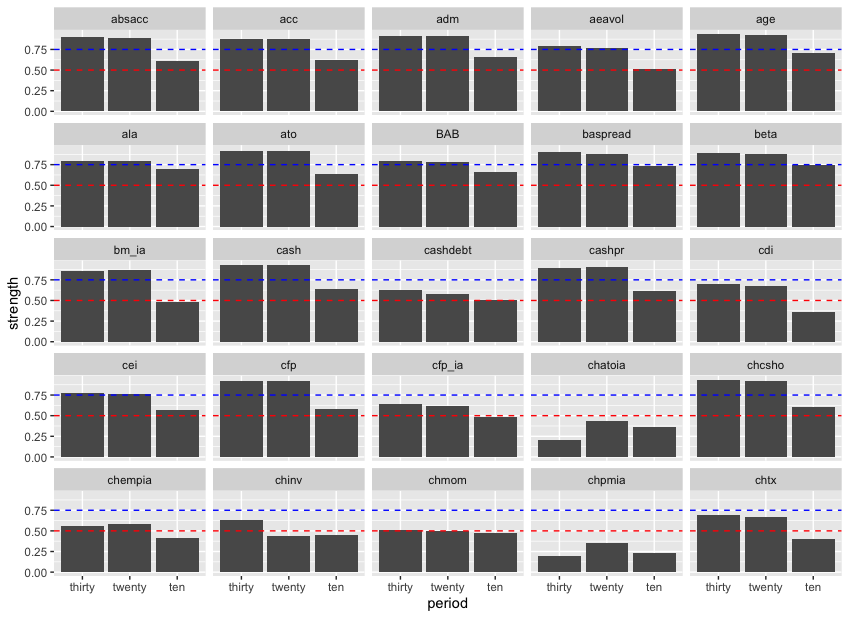
\includegraphics[scale = 0.75]{strength_comparison_I}
\end{figure}
\end{landscape}



\begin{landscape}
\begin{figure}[ht]
		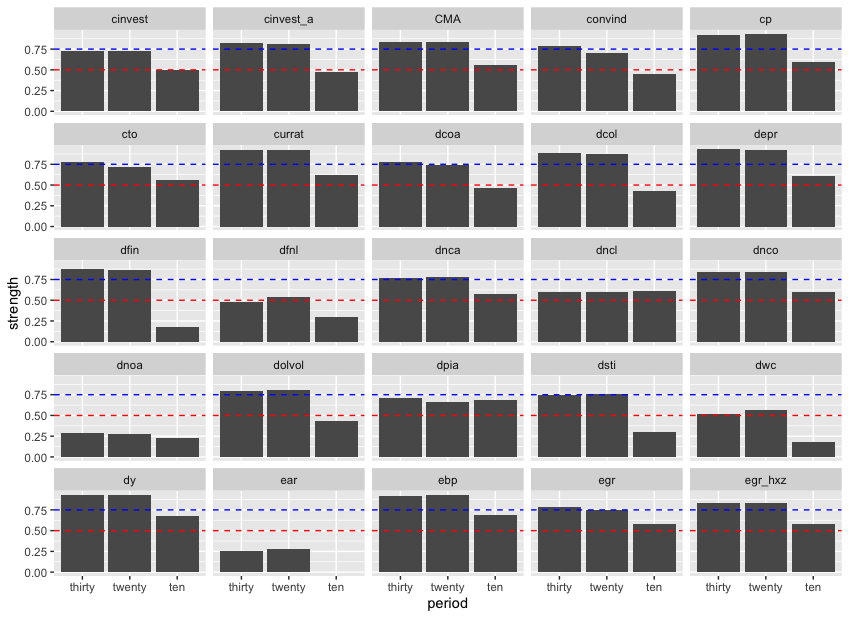
\includegraphics[scale = 0.75]{strength_comparison_II}
		\centering
	\end{figure}
\end{landscape}

\begin{landscape}
	\begin{figure}[ht]
		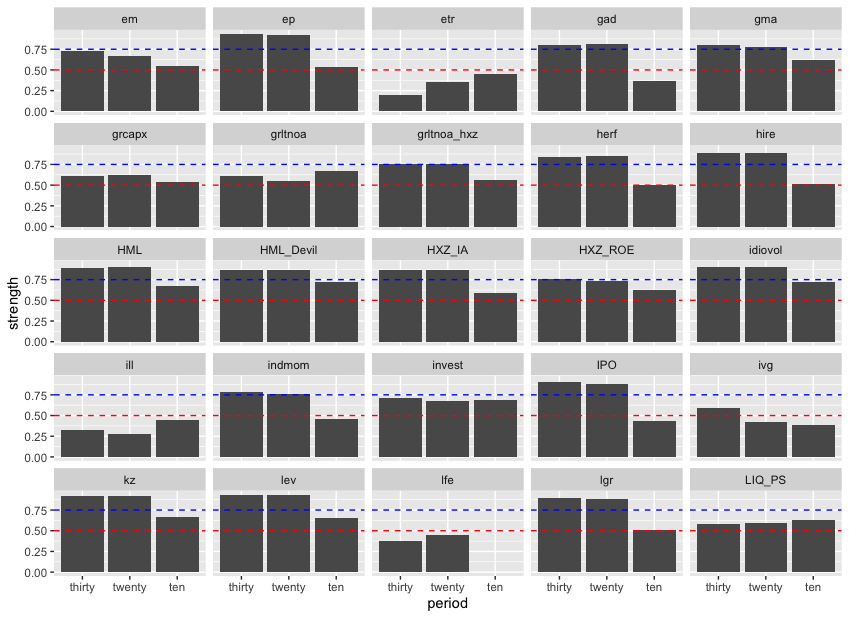
\includegraphics[scale = 0.75]{strength_comparison_III}
		\centering
	\end{figure}
\end{landscape}

\begin{landscape}
	\begin{figure}[ht]
		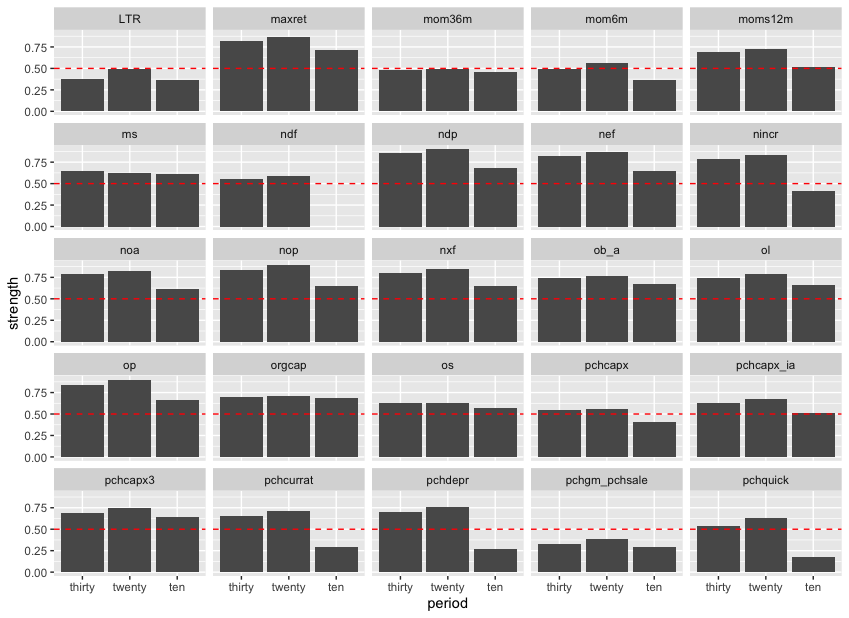
\includegraphics[scale = 0.75]{strength_comparison_IV}
		\centering
	\end{figure}
\end{landscape}

\begin{landscape}
	\begin{figure}[ht]
		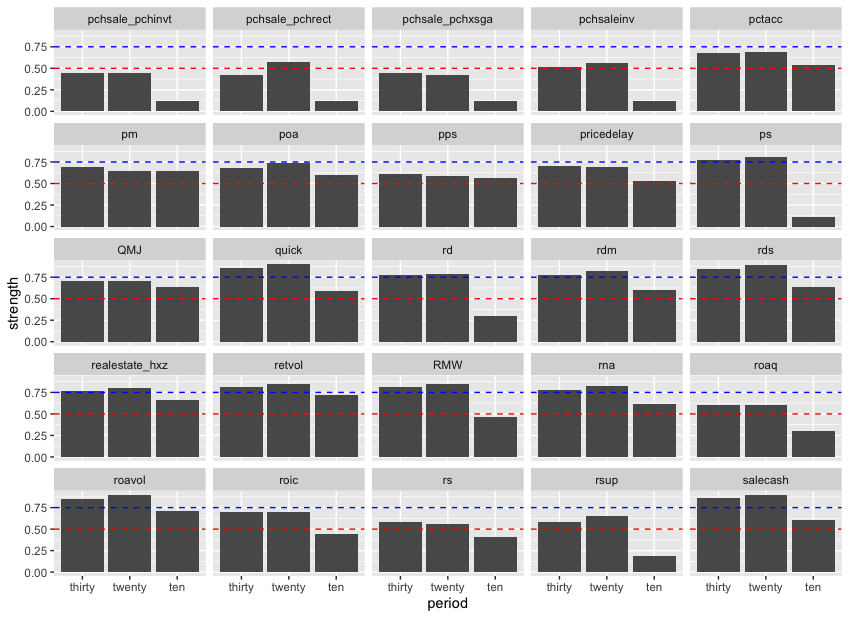
\includegraphics[scale = 0.75]{strength_comparison_V}
		\centering
	\end{figure}
\end{landscape}

\begin{landscape}
	\begin{figure}[ht]
		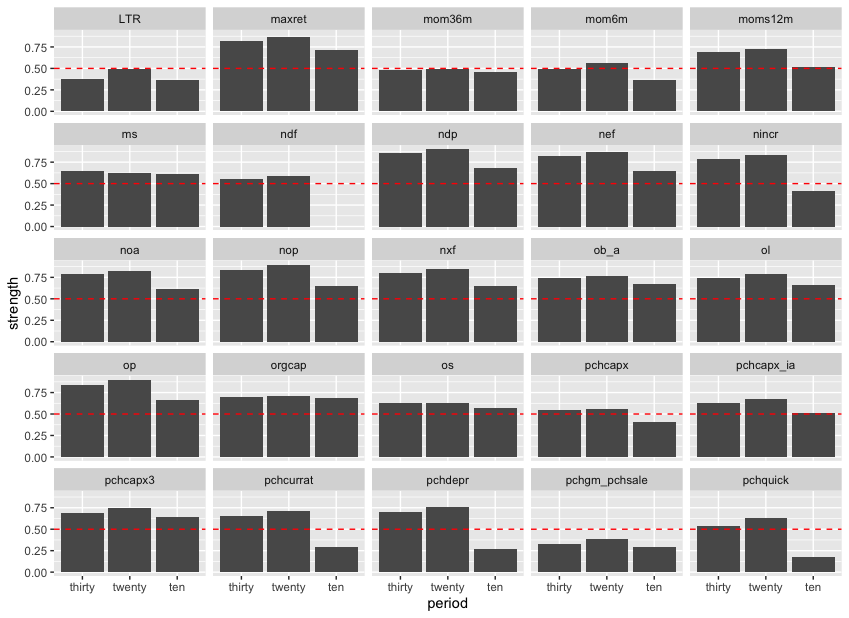
\includegraphics[scale = 0.75]{strength_comparison_IV}
		\centering
		\begin{minipage}{\textwidth}
			{\footnotesize {\bf Notes:} The figure compare the strength of every factor's strength in different data set. The x-axis indicates the data set: thirty is thirty years data set (January 1987 to December 2017), twenty is twenty year data set (January 1997 to December 2017), and ten is ten year data set (January 2007 to December 2017). The red dash line and blue dash line represent 0.5 and 0.75 threshold value respectively.}
		\end{minipage}
	\end{figure}
\end{landscape}

\begin{landscape}
	\begin{figure}[ht]
		\centering
		\caption{Thirty Year Decompose Comparison}\label{figure:thirty_decompose}
		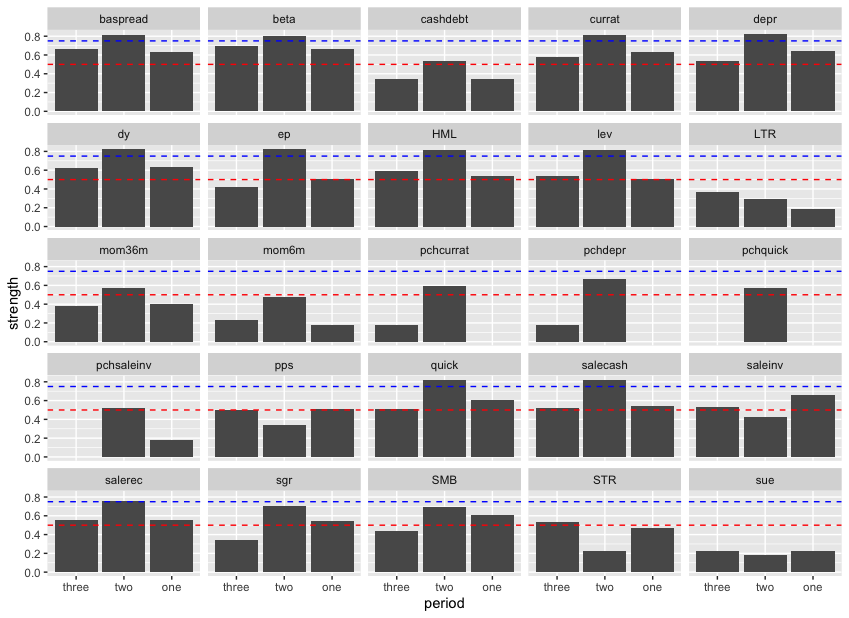
\includegraphics[scale = 0.75]{thirty_decompose_I}
	\end{figure}
\end{landscape}


\begin{landscape}
	\begin{figure}[ht]
		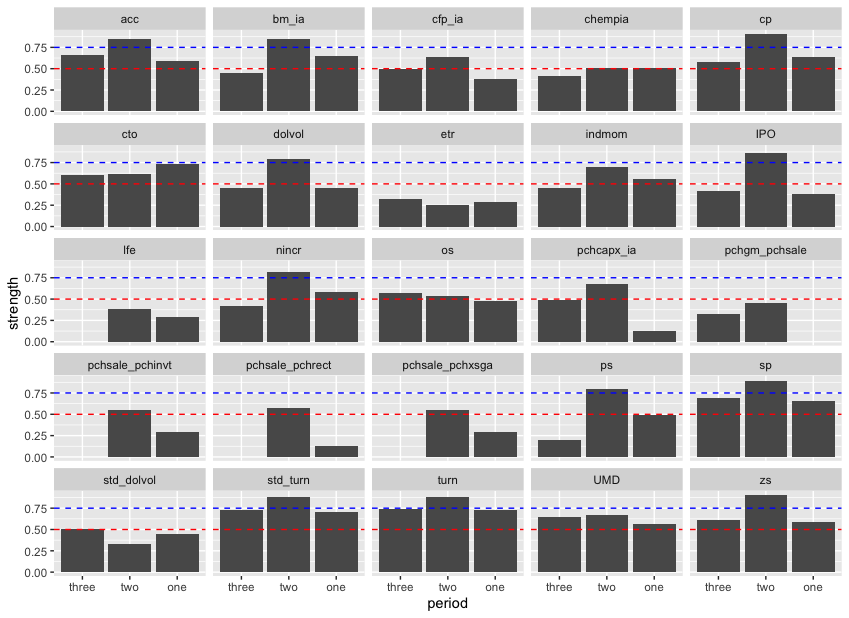
\includegraphics[scale = 0.75]{thirty_decompose_II}
		\centering
	\end{figure}
\end{landscape}

\begin{landscape}
	\begin{figure}[ht]
		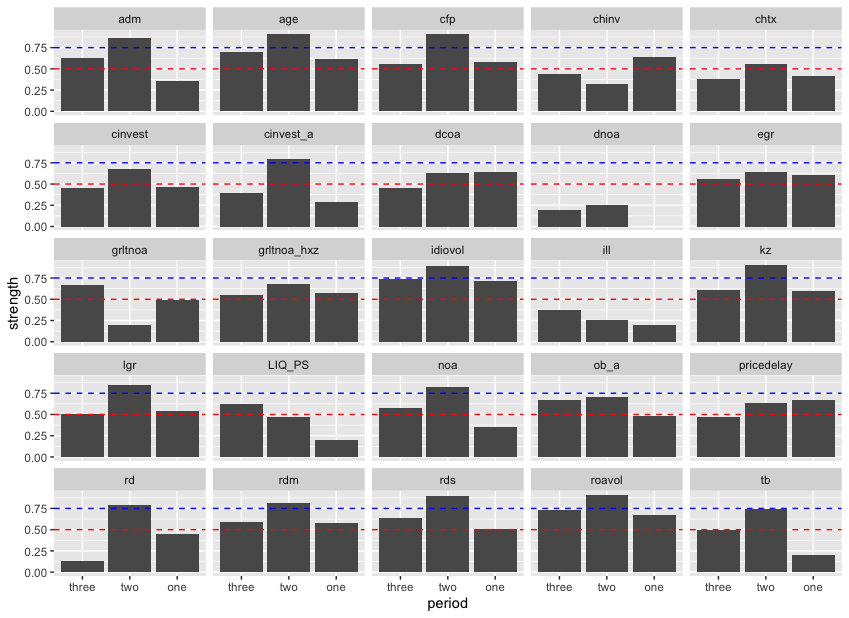
\includegraphics[scale = 0.75]{thirty_decompose_III}
		\centering
	\end{figure}
\end{landscape}

\begin{landscape}
	\begin{figure}[ht]
		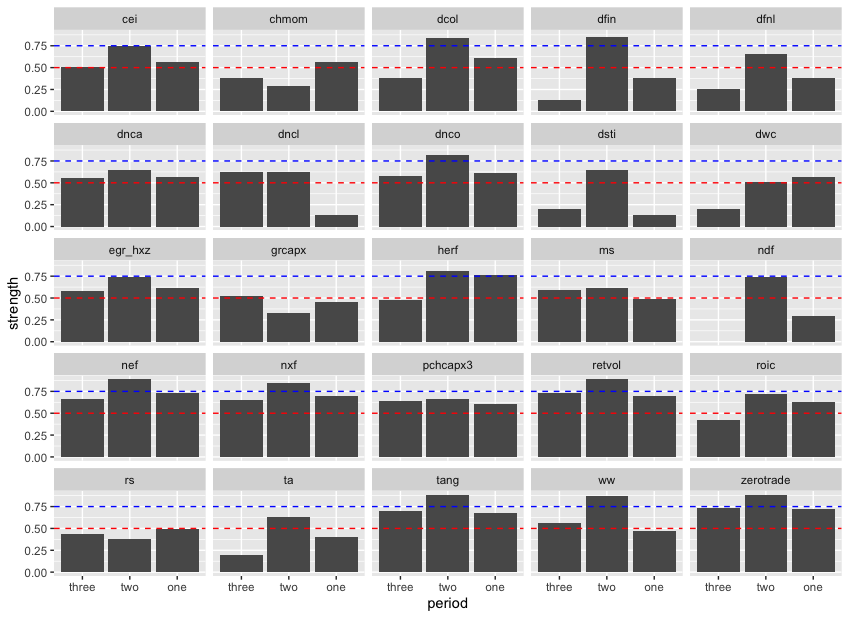
\includegraphics[scale = 0.75]{thirty_decompose_IV}
		\centering
	\end{figure}
\end{landscape}

\begin{landscape}
	\begin{figure}[ht]
		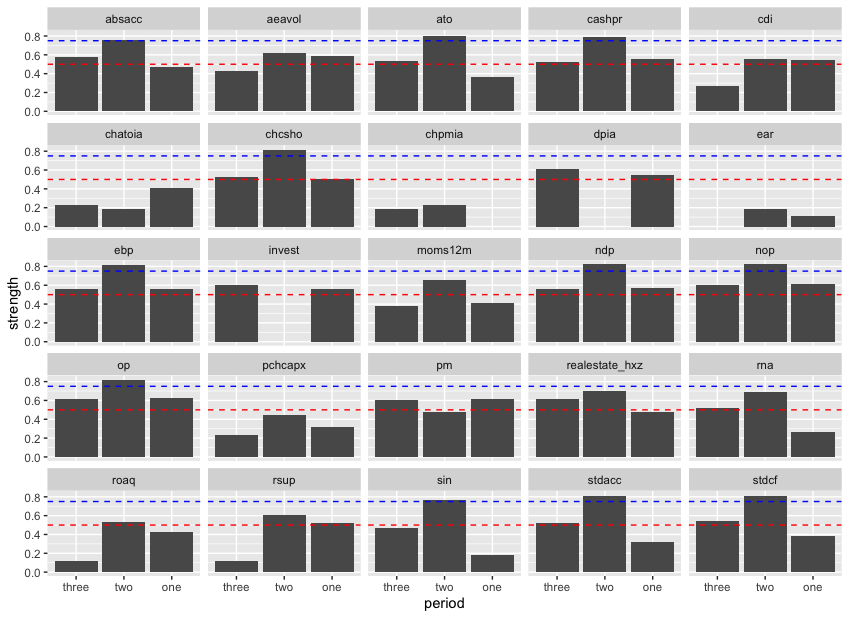
\includegraphics[scale = 0.75]{thirty_decompose_V}
		\centering
	\end{figure}
\end{landscape}

\begin{landscape}
	\begin{figure}[ht]
		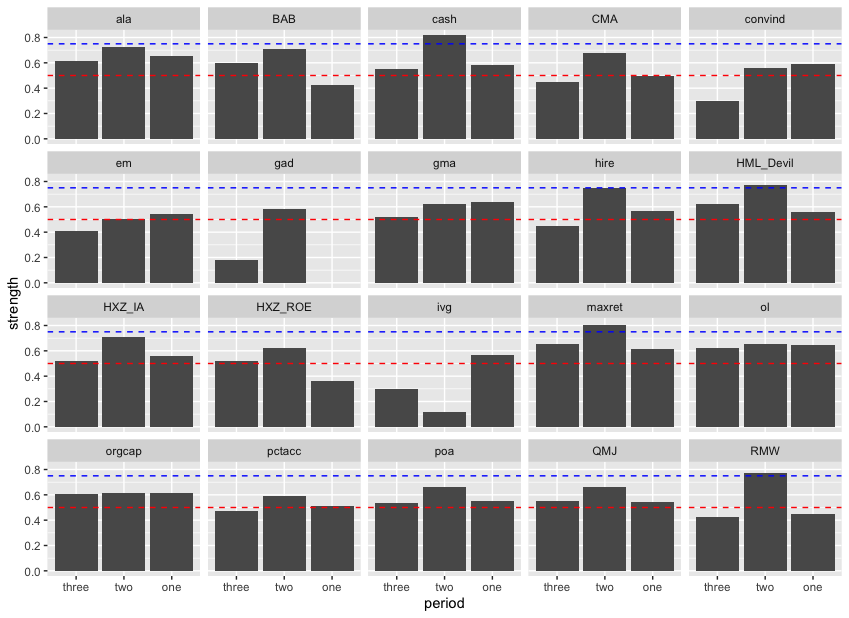
\includegraphics[scale = 0.75]{thirty_decompose_VI}
		\centering
		\begin{minipage}{\textwidth}
			{\footnotesize {\bf Notes:} The figure compare the strength of factor using subsample from the thirty year data.. The x-axis indicates the subsample data set: three is third decade (January 2007 to December 2017), two is second decade (January 1997 to December 2007), and one is the first decade (January 1987 to December 1997). The red dash line and blue dash line represent 0.5 and 0.75 threshold value respectively.}
		\end{minipage}
	\end{figure}
\end{landscape}



\begin{landscape}
	\begin{figure}[ht]
		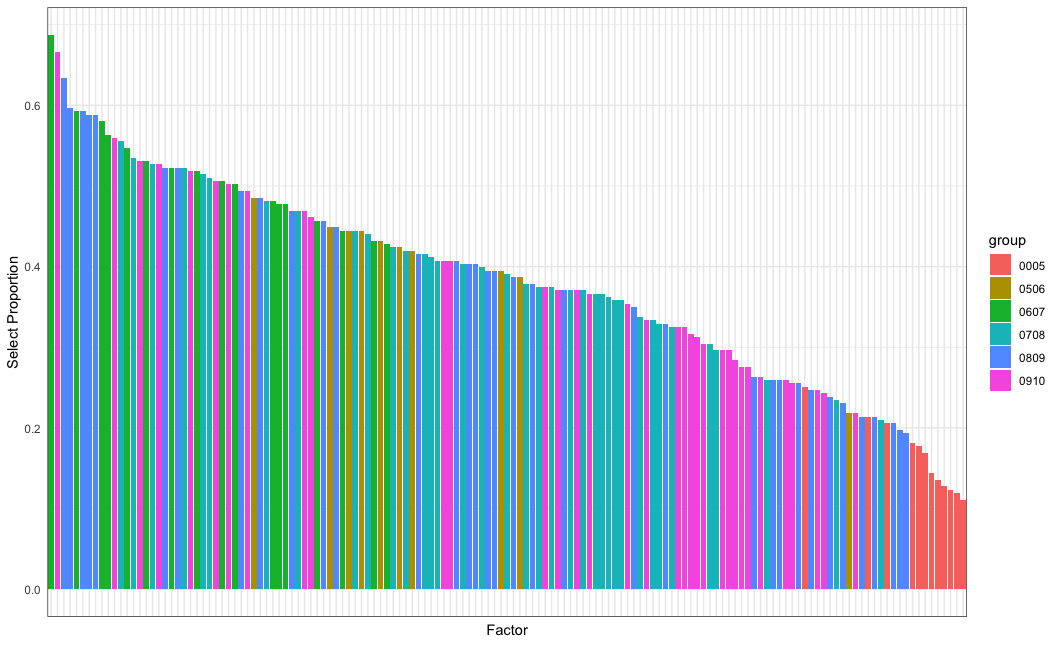
\includegraphics[scale = 0.65]{en_plot}
		\centering
	\end{figure}
\end{landscape}

\begin{landscape}
	\begin{figure}[ht]
		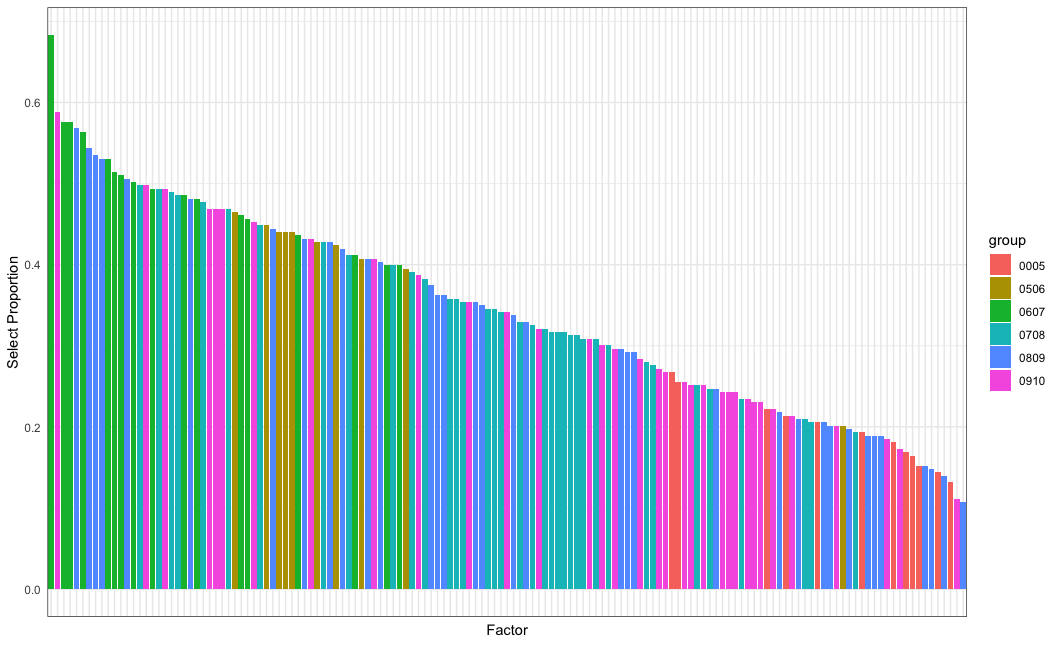
\includegraphics[scale = 0.65]{lasso_plot}
		\centering
	\end{figure}
\end{landscape}

%\begin{landscape}
%	\begin{figure}[ht]
%			\caption{The scatter Plot for three period}\la bel{figure:scatter}
%		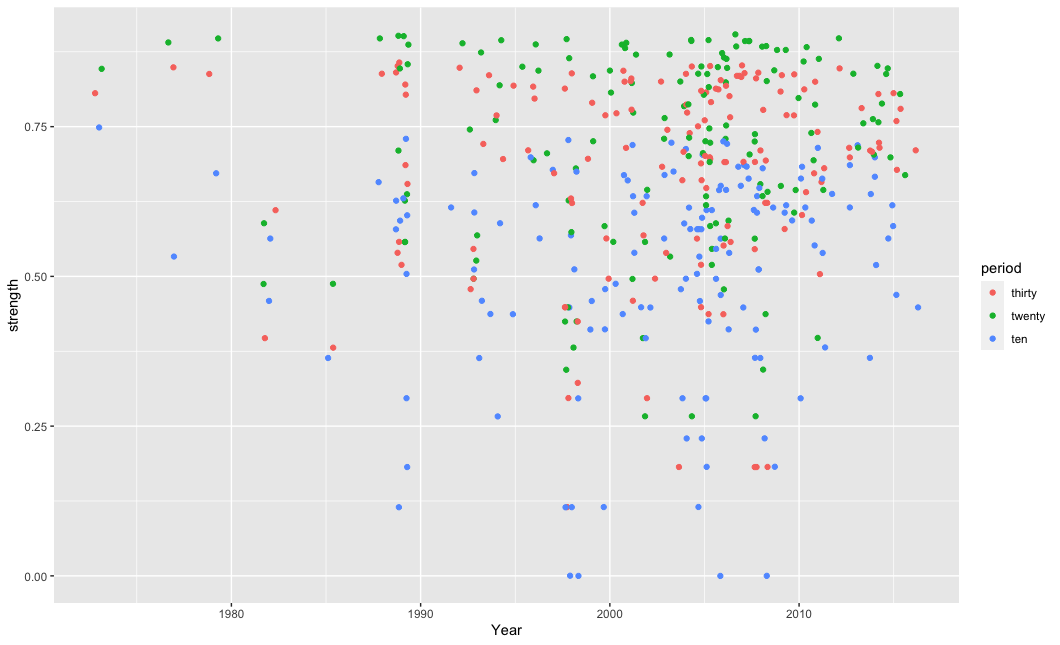
\includegraphics[width=\columnwidth]{scatter}
%		\centering
%					\begin{minipage}{\textwidth}
%			{\footnotesize {\bf Notes:} This scatter plot illustrates the relationship between the factor strength and the factor's publish year. The x-axis represent the year, and the y-axis represent the factor strength. For each factor, we estimate it's strength base on three different data sets, and we use different colour to indicates the three different data set.}
%		\end{minipage}
%	\end{figure}
%\end{landscape}


%\end{document}